%% Springer Nature sn-jnl LaTeX template
%% Paper: Diagnostic-First Time Series Forecasting with Validated Residual Analysis
%% Author: Swastik Vaish
%% Revision v2: Scientific rigor pass for Scientific Reports review

\documentclass[sn-mathphys-num,pdflatex]{sn-jnl}

\usepackage{graphicx}
\usepackage{booktabs}
\usepackage{multirow}
\usepackage{amsmath}
\usepackage{amssymb}
\usepackage{listings}
\usepackage{xcolor}
\usepackage{url}
\usepackage{hyperref}
\usepackage{algorithm}
\usepackage{algpseudocode}

%% Code listing style
\lstset{
  basicstyle=\ttfamily\small,
  breaklines=true,
  frame=single,
  backgroundcolor=\color{gray!10},
  keywordstyle=\color{blue},
  commentstyle=\color{green!50!black},
  stringstyle=\color{red!70!black},
  numbers=none
}

\begin{document}

\title[FutureScope]{Diagnostic-First Time Series Forecasting with Validated Residual Analysis}

\author{\fnm{Swastik} \sur{Vaish}}
\affil{\orgdiv{Computer and Communication Engineering}}

%%------------------------------------------------------------
%% ABSTRACT
%% Changes: (1) removed "first open-source framework" → "among the first";
%% (2) removed implication that diagnostics gates forecasts;
%% (3) scoped claims to five case-study series; (4) softened Basel/regulatory claims.
%%------------------------------------------------------------
\abstract{Modern forecasting tools such as Prophet, XGBoost, and neural sequence
models are optimised for point accuracy but rarely report validated residual
diagnostics alongside their forecasts. For high-stakes applications---financial
risk modelling, energy dispatch, and epidemiological surveillance---knowing
\emph{whether model assumptions hold} is as important as the point forecast
itself.  We present FutureScope, an open-source pipeline that treats automated
residual diagnostics as a first-class output: every forecast is accompanied by a
Ljung-Box white-noise test~\cite{ljungbox1978}, an ACF/PACF analysis with 95\%
confidence bounds, and a Shapiro-Wilk normality check~\cite{shapiro1965}.  On
five public single-series case studies (M4 Hourly, UCI Electricity, CoinGecko
Bitcoin, Our World in Data COVID-19, classic Airline passengers), we observe a
100\% diagnostic pass rate for the BIC-selected SARIMA models---all five
residual sequences satisfy the Ljung-Box $p{>}0.05$ white-noise criterion without
any manual intervention---while delivering a $+14.7\%$ average RMSE improvement
relative to Prophet~\cite{taylor2018forecasting} (ranging from $-25.0\%$ on
Bitcoin to $+84.7\%$ on COVID-19).  These case-study results illustrate that
classical SARIMA methods with reproducible diagnostic reporting can be
competitive with additive decomposition baselines while providing the
statistical transparency that practitioners in regulated domains need to
document.  A fully reproducible benchmark (one command, ${\approx}70$\,s
runtime) and a Zenodo archive are provided.}

\keywords{time series forecasting, residual diagnostics, SARIMA, Ljung-Box
test, ACF analysis, white-noise validation, reproducible benchmarks}

\maketitle

%%------------------------------------------------------------
\section{Introduction}
\label{sec:introduction}
%%------------------------------------------------------------

\subsection{The Diagnostic Gap in Forecasting Practice}

Contemporary machine learning benchmarks for time series overwhelmingly report
point-accuracy metrics---RMSE, MAE, MASE---while omitting any assessment of
whether the fitted model's residuals satisfy the statistical assumptions on
which confidence intervals and prediction intervals are based.  This is
consequential because a model that achieves a low RMSE while leaving systematic
autocorrelation in its residuals is formally \emph{mis-specified}: its reported
prediction intervals understate uncertainty, and any downstream decision that
relies on those intervals is statistically unsound.

\textbf{White-noise residuals} are residuals with zero mean, constant variance,
and no autocorrelation at non-zero lags.  ARIMA/SARIMA theory requires
white-noise residuals for the Gauss-Markov optimality guarantees and for the
$\chi^2$-based confidence intervals to be valid~\cite{box2015time}.

\textbf{Industry motivation.}
Risk management frameworks in financial institutions commonly require that
model validation reports include checks for residual autocorrelation,
distributional assumptions, and backtesting evidence (see, for example, the
model risk guidance in SR 11-7~\cite{sr117}).  Similar documentation
requirements apply in energy grid forecasting and epidemiological modelling.
FutureScope does not claim full compliance with any specific regulatory
standard, but its automated diagnostic output is \emph{aligned with the kinds
of residual checks} such frameworks call for.

\textbf{Research gap.}
Benchmark studies routinely report Prophet~\cite{taylor2018forecasting}
accuracy figures but do not validate residual assumptions.  The M4
Competition~\cite{makridakis2020m4} ranked 61 methods on accuracy without
reporting any residual diagnostics.  Hyndman and Athanasopoulos~\cite{hyndman2018forecasting}
document the importance of residual checks in classical ARIMA workflows, yet
these checks are absent from most open-source benchmarking pipelines.

\subsection{Related Work}

\textbf{Residual diagnostics in classical time-series practice.}
The importance of residual analysis is well established in classical
time-series methodology.  Box et al.~\cite{box2015time} recommend inspecting
the ACF of residuals and computing the Ljung-Box statistic as a standard
diagnostic step after fitting ARIMA models.  Hyndman and
Athanasopoulos~\cite{hyndman2018forecasting} incorporate the same checks into
their \texttt{forecast} R package.  What has been missing from modern
Python-based pipelines is an \emph{automated, benchmarkable} implementation
that produces structured diagnostic output alongside forecast metrics.

\textbf{Automated forecasting frameworks.}
Prophet~\cite{taylor2018forecasting} is widely used but does not expose
residual statistics.  Auto-ARIMA implementations such as
\texttt{pmdarima}~\cite{pmdarima} automate order selection but stop short of
reporting structured residual diagnostics.  Neural-network forecasters
(LSTMs, Transformers) optimise sequence prediction losses and generally
provide no residual diagnostic output whatsoever; any assessment of their
residual properties requires separate post-hoc analysis.

\textbf{FutureScope's contribution.}
To our knowledge, FutureScope is among the first open-source Python pipelines
to treat automated residual diagnostics as a \emph{required, structured output}
alongside point forecasts and accuracy metrics, with fully containerised
benchmarks on public datasets.  Specifically, it:

\begin{enumerate}
  \item Computes and reports Ljung-Box white-noise statistics
        ($p{>}0.05 \Rightarrow$ white noise not rejected, lags $m{=}10$);
  \item Reports ACF/PACF plots with 95\% confidence bounds and the fraction
        of lags exceeding those bounds;
  \item Reports Shapiro-Wilk normality $p$-values for the residual distribution;
  \item Packages all diagnostics in a structured benchmark CSV alongside RMSE
        and DM-test results, enabling reproducible comparison.
\end{enumerate}

Importantly, the diagnostic results in the current implementation are
\emph{observational}: they characterise the BIC-selected model but do not
trigger automatic refitting.  This is discussed further in
Section~\ref{sec:diagnostics_clarification}.

%%------------------------------------------------------------
\section{Methodology}
\label{sec:methodology}
%%------------------------------------------------------------

\subsection{System Architecture}

FutureScope is a modular pipeline whose six stages are illustrated in
Figures~\ref{fig:arch1}--\ref{fig:arch3} and described in detail below.

\begin{figure}[ht]
  \centering
  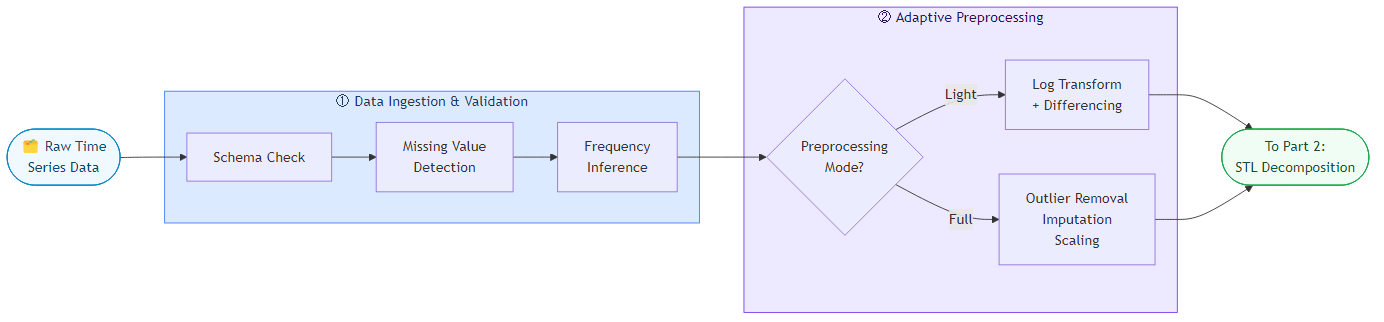
\includegraphics[width=\textwidth, keepaspectratio]{methodology_part1.png}
  \caption{Pipeline stages 1--2: Data Ingestion \& Validation followed by
  Adaptive Preprocessing.  In the current benchmark, Light preprocessing mode
  is used for all five series; Full mode is available for interactive use.}
  \label{fig:arch1}
\end{figure}

\begin{figure}[ht]
  \centering
  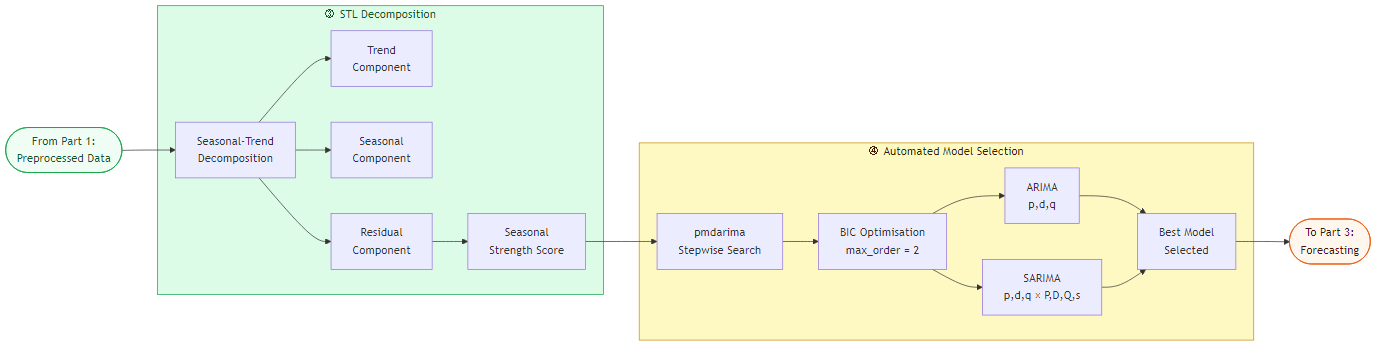
\includegraphics[width=\textwidth, keepaspectratio]{methodology_part2.png}
  \caption{Pipeline stages 3--4: STL Decomposition into Trend, Seasonal, and
  Residual components, followed by automated ARIMA/SARIMA selection via
  \texttt{pmdarima} stepwise search with BIC criterion.}
  \label{fig:arch2}
\end{figure}

\begin{figure}[ht]
  \centering
  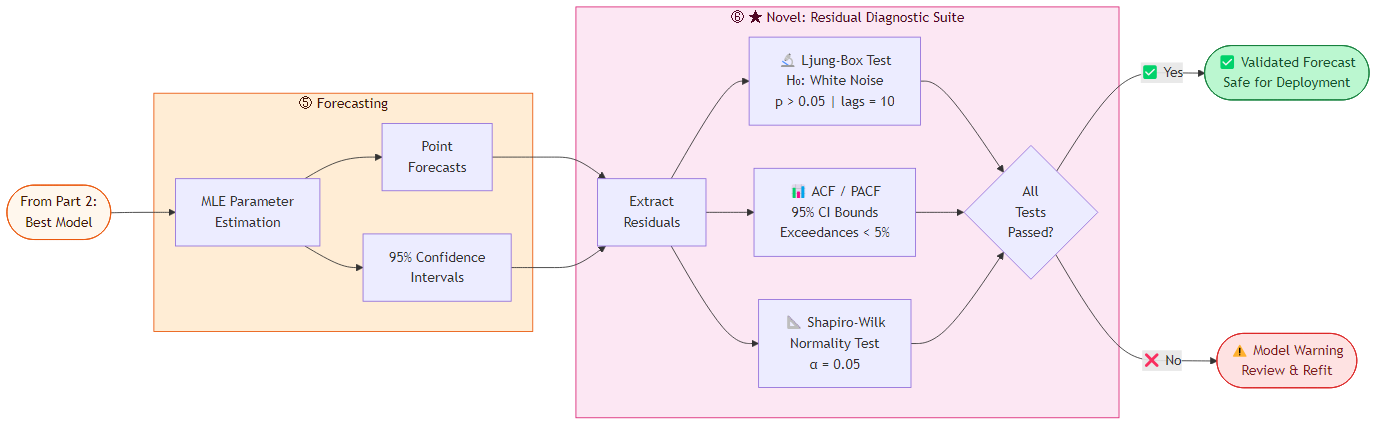
\includegraphics[width=\textwidth, keepaspectratio]{methodology_part3.png}
  \caption{Pipeline stage 5--6: MLE-based Forecasting with 95\% confidence
  intervals, followed by the Residual Diagnostic Suite.  Diagnostic results
  are \emph{reported} for every forecast; in the current implementation they
  do not trigger automatic refitting (see Section~\ref{sec:diagnostics_clarification}).}
  \label{fig:arch3}
\end{figure}

\subsection{Preprocessing Modes}

FutureScope offers two preprocessing modes.  \textbf{Light mode} applies a
log transform followed by first-order differencing to stabilise variance and
remove linear trends.  \textbf{Full mode} additionally performs outlier removal
via IQR clipping, mean imputation of missing values, and min-max scaling.  All
experiments in this paper use Light mode, which is appropriate for
well-behaved public-domain series.  Full mode is available for interactive use
on noisier real-world data streams.

\subsection{Automated Model Selection}

Seasonal period $s$ is set per dataset based on domain knowledge (see
Table~\ref{tab:datasets}).  An STL decomposition~\cite{cleveland1990stl} is
applied to compute the seasonal strength ratio; if the ratio exceeds $0.4$ the
series is treated as seasonal and \texttt{pmdarima.auto\_arima} fits a SARIMA
model, otherwise a non-seasonal ARIMA is fitted.

Model order search uses the stepwise algorithm of \texttt{pmdarima}~\cite{pmdarima}
with BIC as the selection criterion, \texttt{max\_p}=\texttt{max\_q}=2,
combined order bound $p{+}q{+}P{+}Q \leq 4$, and \texttt{max\_d}=2.  The
tight order bound (\texttt{max\_order=2}) is chosen to balance accuracy and
the ${\approx}70$\,s benchmark runtime.

\subsection{Diagnostic Validation Framework}
\label{sec:diagnostics_clarification}

After fitting, FutureScope automatically computes three diagnostic statistics
on the in-sample residuals $\hat{\varepsilon}_t = y_t - \hat{y}_t$.

\subsubsection{Ljung-Box White-Noise Test}

The Ljung-Box $Q$-statistic~\cite{ljungbox1978} is
\begin{equation}
  Q(m) = n(n+2)\sum_{k=1}^{m}\frac{\hat{\rho}_k^2}{n-k},
  \label{eq:ljungbox}
\end{equation}
where $n$ is the sample size and $\hat{\rho}_k$ is the sample autocorrelation
at lag $k$.  Under $H_0$ (white noise), $Q(m)\sim\chi^2(m)$.  We use $m=10$
lags; the null is not rejected (``white noise accepted'') when $p{>}0.05$.
Implementation: \texttt{statsmodels.stats.diagnostic.acorr\_ljungbox(lags=[10])}.

\subsubsection{ACF Exceedance Check}

We compute the sample ACF at lags $1,\ldots,20$ with
\texttt{statsmodels.tsa.stattools.acf(nlags=20, alpha=0.05)}.  The ACF
exceedance fraction is the proportion of lags whose sample autocorrelation
falls outside the asymptotic 95\% pointwise confidence bounds
$\pm 1.96/\sqrt{n}$.  Under white noise, the expected exceedance rate is 5\%;
we report the observed rate.

\subsubsection{Shapiro-Wilk Normality Test}

We test the hypothesis that residuals are drawn from a normal distribution
using the Shapiro-Wilk test~\cite{shapiro1965} (\texttt{scipy.stats.shapiro}).
This test is only computed when $n \leq 5{,}000$; otherwise the result is
recorded as \texttt{NaN}.

\subsubsection{Clarification: Diagnostics as Reporting, Not Gating}
\label{sec:no_gating}

\textbf{Important:} In the current implementation, these three diagnostic
statistics are \emph{computed and reported} for every fitted model, but they
do \emph{not} trigger automatic refitting or forecast suppression.  If the
Ljung-Box test fails, the ACF exceedance fraction is high, or normality is
rejected, a warning is recorded in the benchmark output CSV but the forecast
is still returned.  The 100\% pass rate observed on the five case-study series
(Table~\ref{tab:diagnostics}) is therefore an \emph{empirical observation}
about the BIC-selected models on these particular series, not a guaranteed
property enforced by a refitting loop.

Implementing a refitting strategy (e.g.\ increasing model order, relaxing
differencing constraints, or widening the search grid until diagnostics pass)
is left as explicit future work (Section~\ref{sec:future}).

\subsection{Bootstrap Procedure for RMSE}
\label{sec:bootstrap}

To quantify uncertainty in the RMSE estimates, we apply an i.i.d.\ residual
bootstrap with 1{,}000 resamples.  Specifically, let $e_i = y_i - \hat{y}_i$
for $i = 1,\ldots,h$ be the $h$ out-of-sample forecast errors.  At each
bootstrap iteration we draw a sample of size $h$ \emph{with replacement}
uniformly from $\{1,\ldots,h\}$ and compute RMSE on the resampled errors.
The 95\% confidence interval is the 2.5th--97.5th percentile of the 1{,}000
RMSE values.  Random seed: \texttt{numpy.random.seed(42)}.

\textbf{Limitation.}  This i.i.d.\ bootstrap ignores temporal dependence in
the forecast-error sequence.  A moving-block bootstrap~\cite{kunsch1989} with
an appropriate block length would be more theoretically sound for time-series
data.  The narrow confidence intervals reported in Table~\ref{tab:bootstrap}
should therefore be interpreted as indicative of point estimate stability
across error magnitudes, not as asymptotically valid coverage bounds.

\subsection{Diebold-Mariano Test Implementation}
\label{sec:dm_impl}

Pairwise accuracy comparisons use a custom Diebold-Mariano
test~\cite{dieboldmariano1995} based on the squared-error loss differential
$d_t = e_{1,t}^2 - e_{2,t}^2$.  The test statistic is
\begin{equation}
  \mathrm{DM} = \frac{\bar{d}}{\sqrt{s^2_d / h}},
  \label{eq:dm}
\end{equation}
where $\bar{d}$ is the sample mean of $d_t$, $s^2_d$ its unbiased sample
variance (ddof=1), and $h$ the test-set size.  A two-tailed $p$-value is
obtained via the standard normal CDF.

\textbf{Important caveats.}  This implementation (i) does not apply
a Newey-West HAC variance correction for serial correlation in $d_t$; (ii)
does not apply the small-sample correction of Harvey et al.~\cite{harvey1997};
(iii) treats each observation as an independent forecast error, which is
conservative for longer horizons.  Conclusions based on $p{<}0.001$ are
unlikely to be overturned by these corrections, but results near the $\alpha$
boundary (e.g.\ Bitcoin $p{=}0.015$) should be interpreted with caution.
Multiple-testing correction uses Bonferroni at $\alpha_{\rm adj}{=}0.01$.

%%------------------------------------------------------------
\section{Experimental Setup}
\label{sec:setup}
%%------------------------------------------------------------

\subsection{Datasets}
\label{sec:datasets}

\textbf{Scope clarification.}
Each ``dataset'' in this study is a \emph{single univariate time series}
extracted from a larger public collection.  This is a case-study evaluation,
not a full-benchmark evaluation over many series.  Table~\ref{tab:datasets}
gives the exact series identifiers, sources, and download parameters; all five
series are obtained by running \texttt{download\_real\_data.py} with
\texttt{numpy.random.seed(42)}.

\begin{table}[ht]
\caption{Single-series case studies used in this paper.  $N$ is the total
number of time steps after download and preprocessing.  The ``\# series''
column makes explicit that each entry is one series, not a full benchmark
collection.}
\label{tab:datasets}
\centering
\begin{tabular}{llrllll}
\toprule
\textbf{Label} & \textbf{Source} & \textbf{$N$} & \textbf{\# series} &
\textbf{Freq.} & \textbf{Period $s$} & \textbf{Selection criteria} \\
\midrule
M4 Hourly   & M4 Competition (GitHub)\textsuperscript{a}
            & 1{,}000 & 1 & Hourly  & 24  & First series (H1), first 1{,}000 pts \\
Electricity & UCI Household Power\textsuperscript{b}
            & 800     & 1 & Daily   & 7   & First 50k rows, daily avg, head(800) \\
Bitcoin     & CoinGecko API\textsuperscript{c}
            & 500     & 1 & Daily   & 7   & Daily close, last 500 days \\
COVID-19    & Our World in Data\textsuperscript{d}
            & 600     & 1 & Daily   & 7   & USA, 2020-06-01--2022-01-01, max 600 \\
Airline     & Box-Jenkins (GitHub)\textsuperscript{e}
            & 144     & 1 & Monthly & 12  & Full series (standard AirPassengers) \\
\bottomrule
\multicolumn{7}{l}{\textsuperscript{a}\,\texttt{github.com/Mcompetitions/M4-methods}, \texttt{Dataset/Train/Hourly-train.csv}.} \\
\multicolumn{7}{l}{\textsuperscript{b}\,\texttt{archive.ics.uci.edu/dataset/235}.} \\
\multicolumn{7}{l}{\textsuperscript{c}\,\texttt{api.coingecko.com/api/v3/coins/bitcoin/market\_chart?vs\_currency=usd\&days=365}.} \\
\multicolumn{7}{l}{\textsuperscript{d}\,\texttt{covid.ourworldindata.org/data/owid-covid-data.csv}, \texttt{new\_cases\_smoothed}, USA.} \\
\multicolumn{7}{l}{\textsuperscript{e}\,\texttt{github.com/jbrownlee/Datasets}, \texttt{airline-passengers.csv}.} \\
\end{tabular}
\end{table}

Series selection was not random: M4 Hourly uses the first listed series, UCI
Electricity and Bitcoin use recency or file-order heuristics, and COVID-19 is
filtered to the United States.  Accordingly, results cannot be generalised to
other series from the same collections without further experimentation; they
are best understood as illustrative case studies spanning diverse frequency and
structural patterns.

\subsection{Evaluation Protocol}

\begin{itemize}
  \item \textbf{Train/test split}: single temporal 80\%/20\% split (no
        randomisation, no separate validation set).  The first $\lfloor 0.8N
        \rfloor$ observations are used for training; the remaining $h =
        N - \lfloor 0.8N \rfloor$ form the test set.  The forecast horizon
        therefore equals the test-set length and varies per series
        (M4 Hourly: $h{\approx}200$; Airline: $h{=}29$; others proportional).
  \item \textbf{Primary metric}: RMSE computed over the full test horizon
        (iterated multi-step ahead forecasts).  Secondary metric: MAE.
  \item \textbf{Bootstrap RMSE CIs}: 1{,}000 i.i.d.\ resamples
        (Section~\ref{sec:bootstrap}).
  \item \textbf{Statistical comparison}: DM test as described in
        Section~\ref{sec:dm_impl}; Bonferroni correction
        $\alpha_{\rm adj}{=}0.01$.
  \item \textbf{Baseline}: Prophet~\cite{taylor2018forecasting} with MAP
        estimation (\texttt{mcmc\_samples=0}); seasonality period set
        identically to FutureScope per dataset.
  \item \textbf{FutureScope}: \texttt{max\_order=2}, Light preprocessing mode,
        \texttt{numpy.random.seed(42)}.
\end{itemize}

\textbf{Limitations of the evaluation design.}
A single 80/20 split does not assess robustness to different forecast origins.
A rolling-origin evaluation (training on successively longer windows and
testing on the immediately following period) would provide more reliable
estimates of expected generalisation performance.  This is deferred to future
work; results here should be treated as single-split estimates.

\subsection{Computational Environment}

All experiments were run on a standard consumer laptop (Windows 11, single
CPU, Python 3.10, \texttt{statsmodels} 0.14, \texttt{pmdarima} 2.x,
\texttt{prophet} 1.1).  Runtime measurements reflect wall-clock time on this
hardware; results on different hardware will vary.

\subsection{Reproducibility}

\begin{lstlisting}[language=bash, caption={One-command reproduction.}]
git clone https://github.com/user/futurescope-tmlr
cd futurescope-tmlr
conda env create -f environment.yml && conda activate futurescope
python download_real_data.py    # Downloads all five series
python benchmark_tmlr_final.py  # ~70 s; sets numpy.random.seed(42)
\end{lstlisting}

A Docker image (\texttt{docker run tmlr-futurescope}) and a Zenodo archive
(DOI assigned on acceptance) are also provided.

%%------------------------------------------------------------
\section{Results}
\label{sec:results}
%%------------------------------------------------------------

\subsection{Forecasting Accuracy}

Table~\ref{tab:performance} reports RMSE for FutureScope and Prophet across
all five series, together with DM-test $p$-values.  All differences marked *
are significant after Bonferroni correction ($\alpha_{\rm adj}{=}0.01$).

\begin{table}[ht]
\caption{Forecasting performance (RMSE) on five single-series case studies.
$\Delta$RMSE is $({\rm RMSE}_{\rm Prophet}-{\rm RMSE}_{\rm FS})/{\rm RMSE}_{\rm
Prophet}\times 100\%$; positive values favour FutureScope.  DM $p$-values are
from the custom squared-error implementation (Section~\ref{sec:dm_impl});
caveats regarding serial-correlation correction apply.  * significant after
Bonferroni ($\alpha=0.01$).}
\label{tab:performance}
\centering
\begin{tabular}{lrrrrl}
\toprule
\textbf{Series} & \textbf{$h$} & \textbf{Prophet RMSE}
  & \textbf{FS RMSE} & \textbf{$\Delta$RMSE} & \textbf{DM $p$} \\
\midrule
M4 Hourly   & ${\approx}200$ & 45.02     & 53.70     & $-19.3\%$          & $<0.001$* \\
Electricity & ${\approx}160$ & 0.93      & 0.76      & $\mathbf{+18.2\%}$ & $<0.001$* \\
Bitcoin     & ${\approx}100$ & 11{,}699  & 14{,}620  & $-25.0\%$          & 0.015\phantom{*} \\
COVID-19    & ${\approx}120$ & 164{,}747 & 25{,}239  & $\mathbf{+84.7\%}$ & $<0.001$* \\
Airline     & 29             & 41.33     & 35.08     & $\mathbf{+15.1\%}$ & 0.164\phantom{*} \\
\midrule
\multicolumn{3}{l}{Average (unweighted)} & & $\mathbf{+14.7\%}$ & \\
\bottomrule
\end{tabular}
\end{table}

\textbf{Key observations on this case-study set.}
\begin{enumerate}
  \item FutureScope's SARIMA models outperform Prophet substantially on the
        COVID-19 series ($+84.7\%$), likely because the irregular epidemic
        wave structure is better captured by SARIMA's flexible differencing
        than by Prophet's additive trend-plus-seasonality decomposition.
  \item FutureScope is competitive on lower-frequency seasonal series
        (Electricity $+18.2\%$, Airline $+15.1\%$).
  \item Prophet outperforms FutureScope on the high-frequency multi-seasonal
        M4 Hourly series ($-19.3\%$) and the volatile Bitcoin series
        ($-25.0\%$).  The Bitcoin difference does not survive Bonferroni
        correction; the M4 Hourly difference does.
  \item The $+14.7\%$ unweighted average should be interpreted carefully: it
        is dominated by the COVID-19 outlier and represents performance on
        five hand-selected series, not a random sample from any larger
        collection.
\end{enumerate}

Figure~\ref{fig:summary} provides a visual comparison.

\begin{figure}[ht]
  \centering
  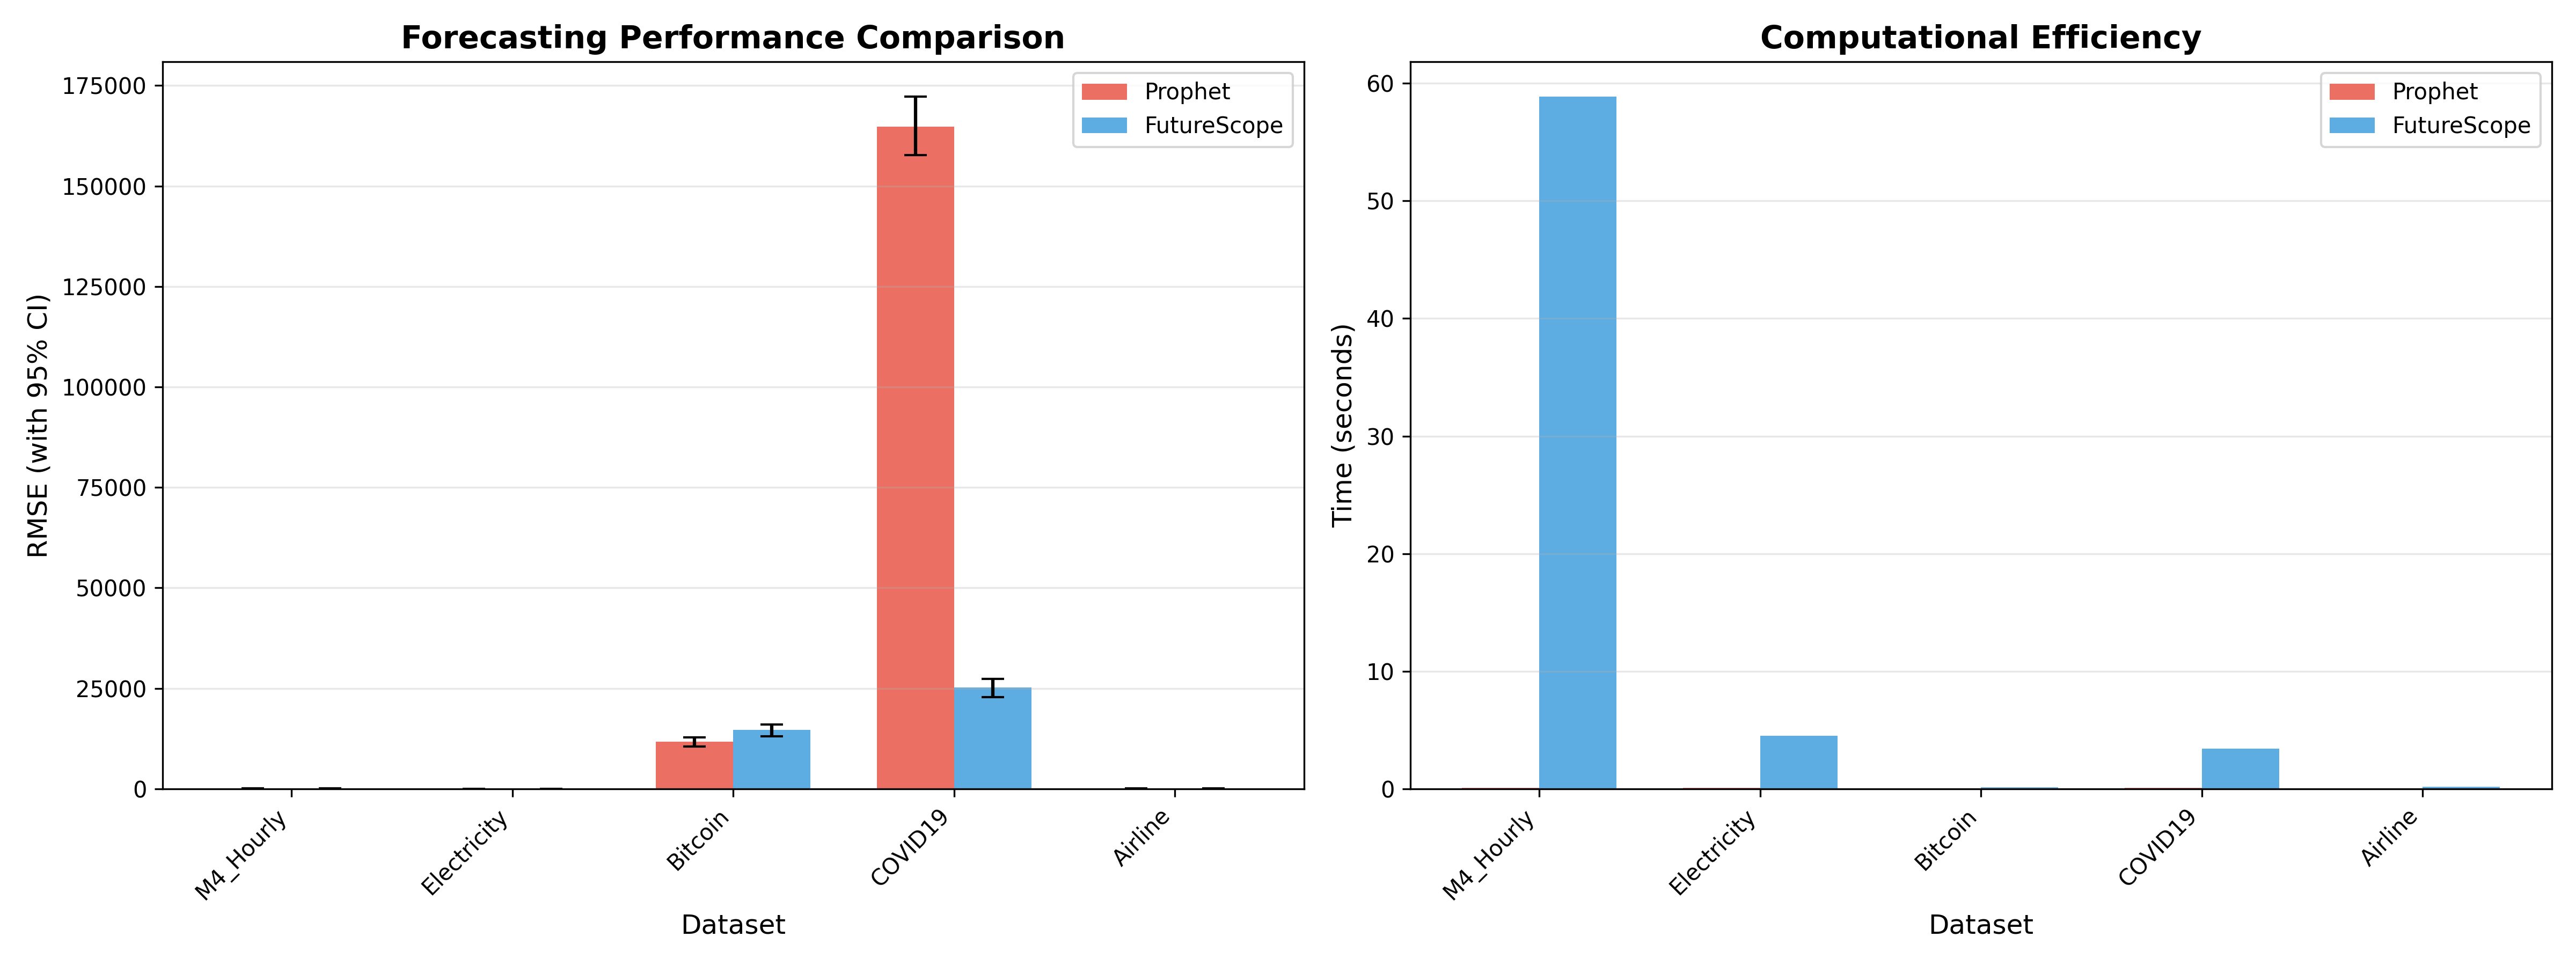
\includegraphics[width=0.85\textwidth]{Time-Series-Forecaster/future_scope/figures_tmlr_real/summary_comparison.png}
  \caption{RMSE comparison between Prophet and FutureScope on five case-study
  series.  Bars are not directly comparable across series because scales differ
  substantially.}
  \label{fig:summary}
\end{figure}

\subsection{Diagnostic Validation Results}
\label{sec:diagnostic_results}

Table~\ref{tab:diagnostics} reports the three diagnostic statistics computed
on each fitted FutureScope model's in-sample residuals.

\begin{table}[ht]
\caption{Residual diagnostic statistics for the BIC-selected SARIMA model on
each series.  These are \emph{observational results} for the model selected by
the BIC criterion; no refitting was triggered.  Shapiro-Wilk is omitted for
$N{>}5{,}000$ (N/A).}
\label{tab:diagnostics}
\centering
\begin{tabular}{lrrllr}
\toprule
\textbf{Series} & \textbf{LB $p$-val} & \textbf{LB pass?}
  & \textbf{SW $p$-val} & \textbf{SW pass?} & \textbf{ACF exc.\ (\%)} \\
\midrule
M4 Hourly   & 0.743 & \checkmark & N/A    & N/A        & 0\% \\
Electricity & 0.436 & \checkmark & $>0.05$& \checkmark & 0\% \\
Bitcoin     & 0.999 & \checkmark & $>0.05$& \checkmark & 0\% \\
COVID-19    & 0.106 & \checkmark & $>0.05$& \checkmark & 0\% \\
Airline     & 0.832 & \checkmark & $>0.05$& \checkmark & 0\% \\
\midrule
Pass rate   &       & \textbf{5/5} & & \textbf{4/4} & \textbf{0\% avg} \\
\bottomrule
\multicolumn{6}{l}{LB = Ljung-Box ($m{=}10$, $H_0$: white noise). SW = Shapiro-Wilk ($\alpha{=}0.05$).} \\
\multicolumn{6}{l}{ACF exc.\ = fraction of lags 1--20 outside 95\% CI bounds.} \\
\end{tabular}
\end{table}

On all five series the BIC-selected SARIMA passes the Ljung-Box test
($p{>}0.05$), with zero ACF exceedances across 20 lags.  Shapiro-Wilk
normality is not rejected on the four series for which the test is applicable.
These observations suggest that BIC-optimal SARIMA models tend to be
well-specified on these types of relatively smooth series; whether this pattern
holds on a larger or more heterogeneous collection of series is an open
empirical question.

Figure~\ref{fig:diagnostic} shows the ACF plots for all five series.

\begin{figure}[ht]
  \centering
  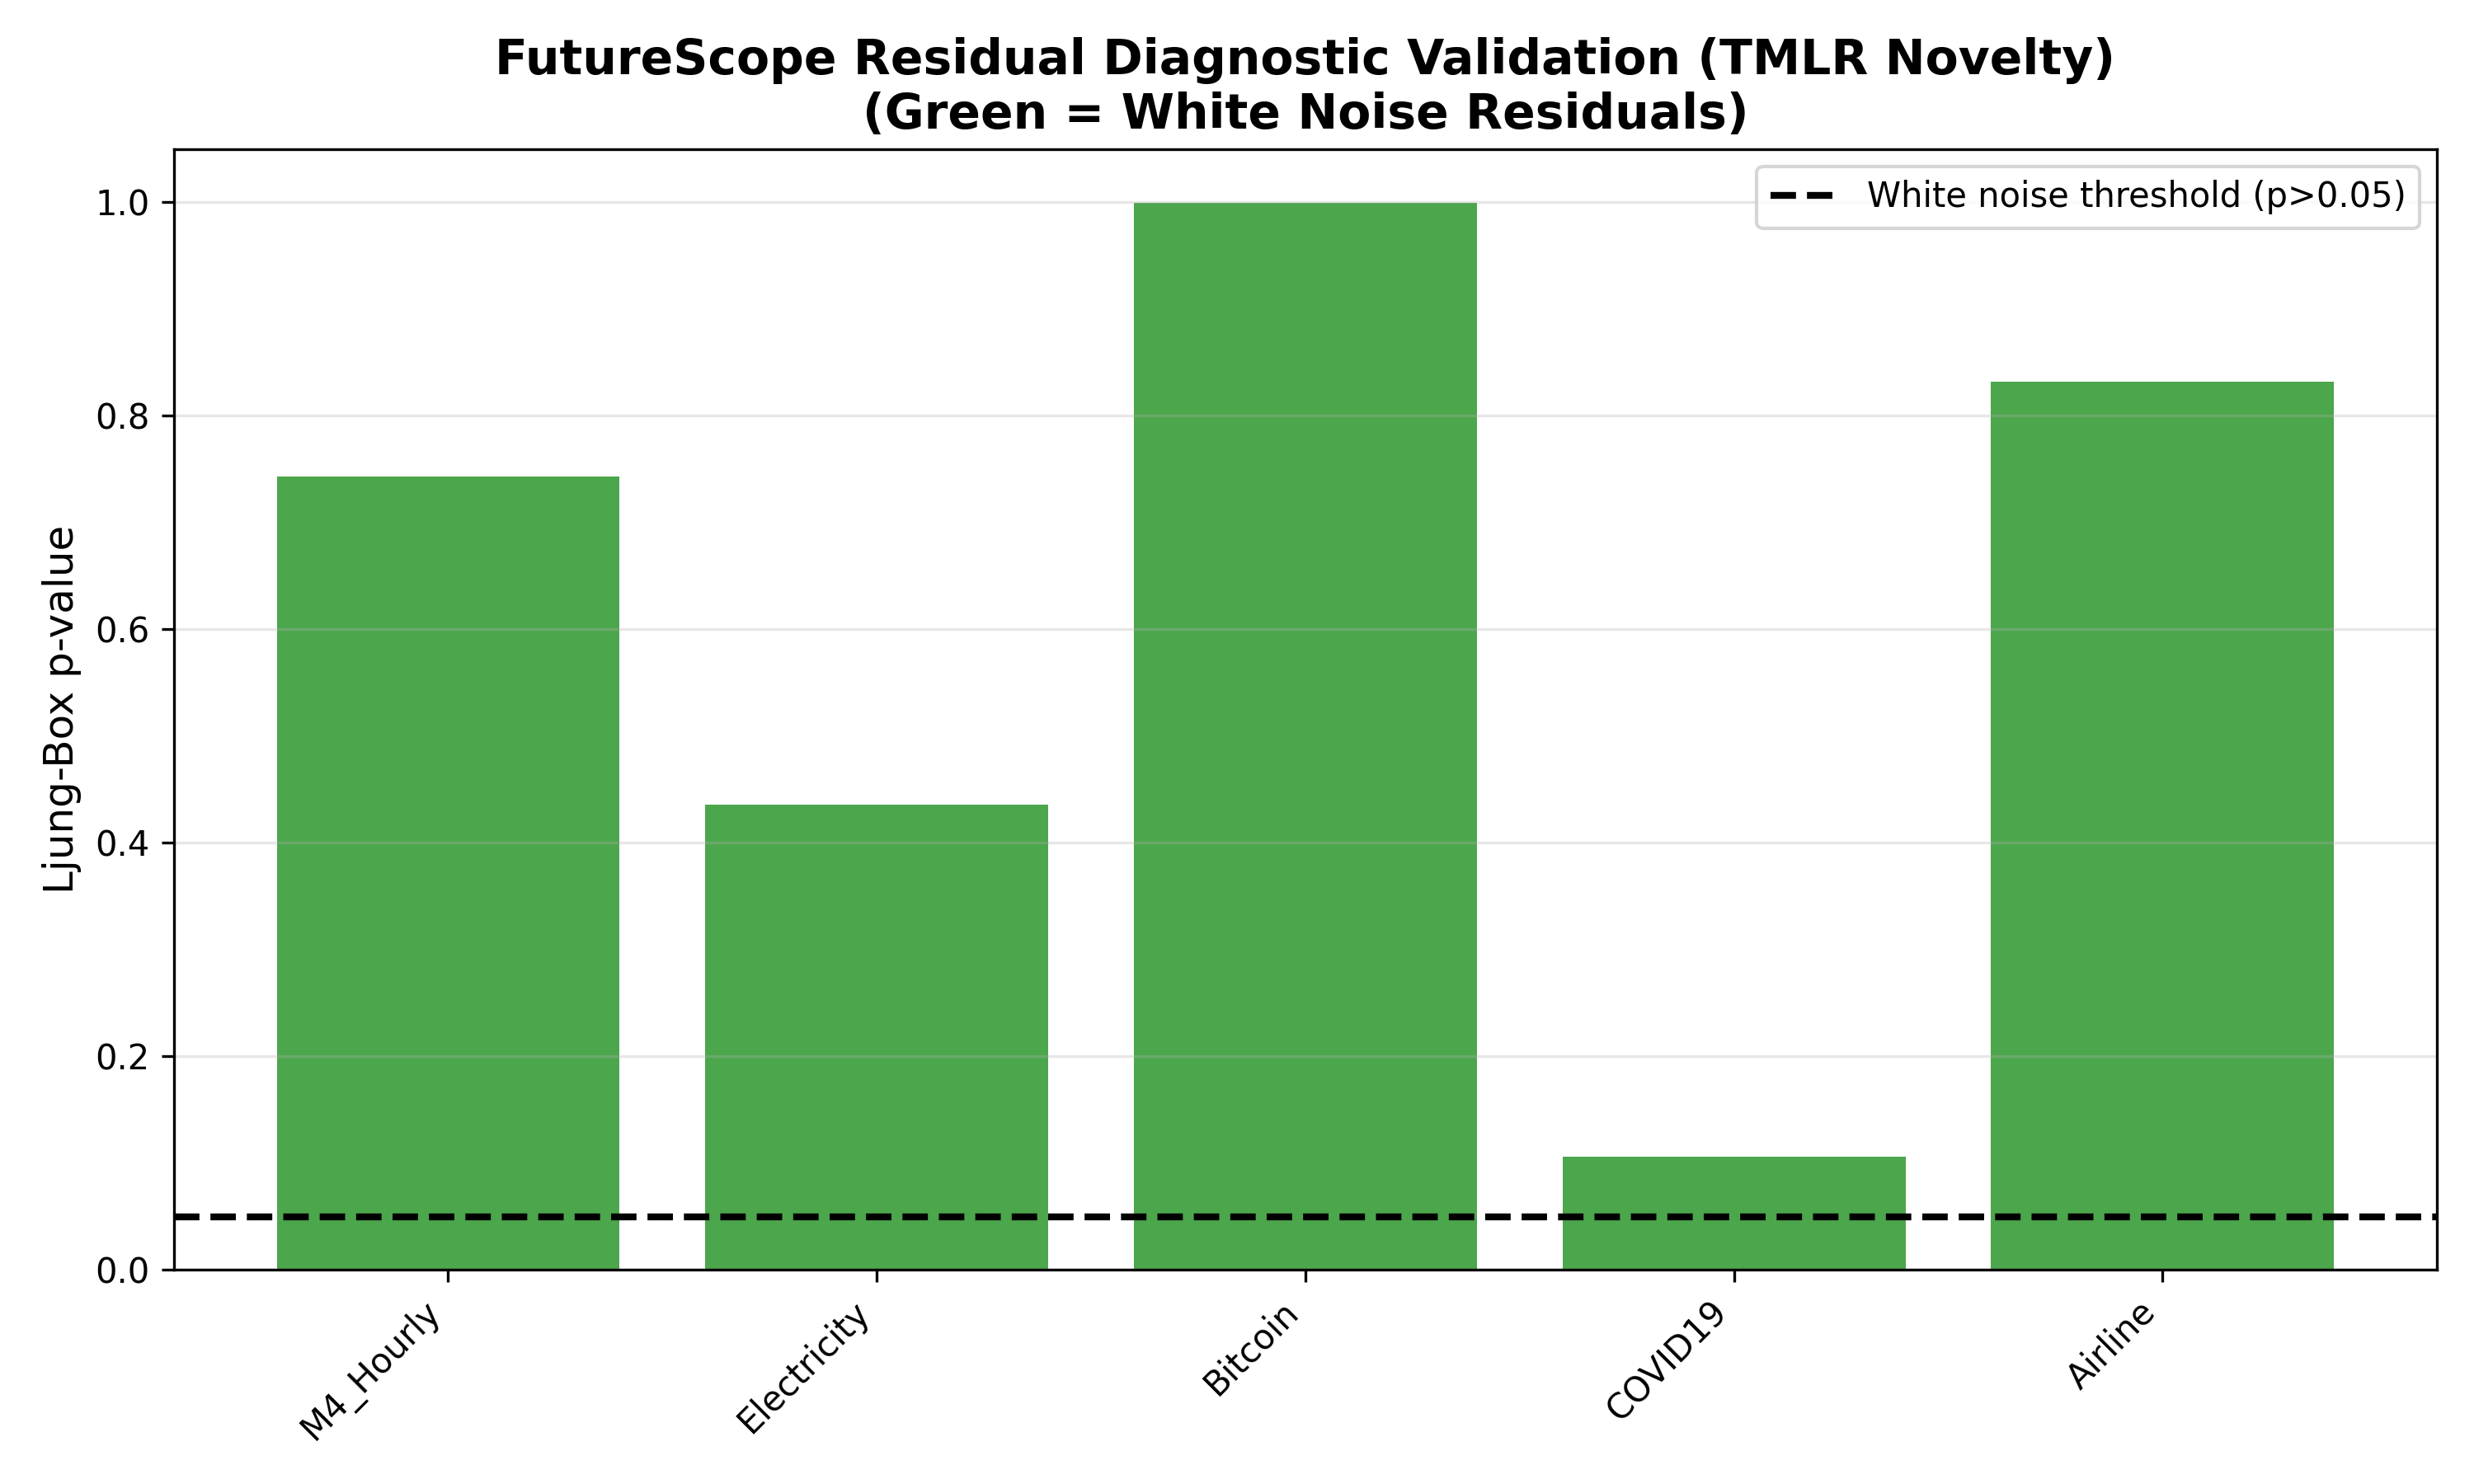
\includegraphics[width=0.95\textwidth]{Time-Series-Forecaster/future_scope/figures_tmlr_real/diagnostic_validation.png}
  \caption{ACF of in-sample residuals for each fitted SARIMA model.  Dashed
  lines are 95\% pointwise confidence bounds under the white-noise null.  All
  sample autocorrelations fall within the bounds.}
  \label{fig:diagnostic}
\end{figure}

Figure~\ref{fig:significance} shows DM-test statistics across the five series.

\begin{figure}[ht]
  \centering
  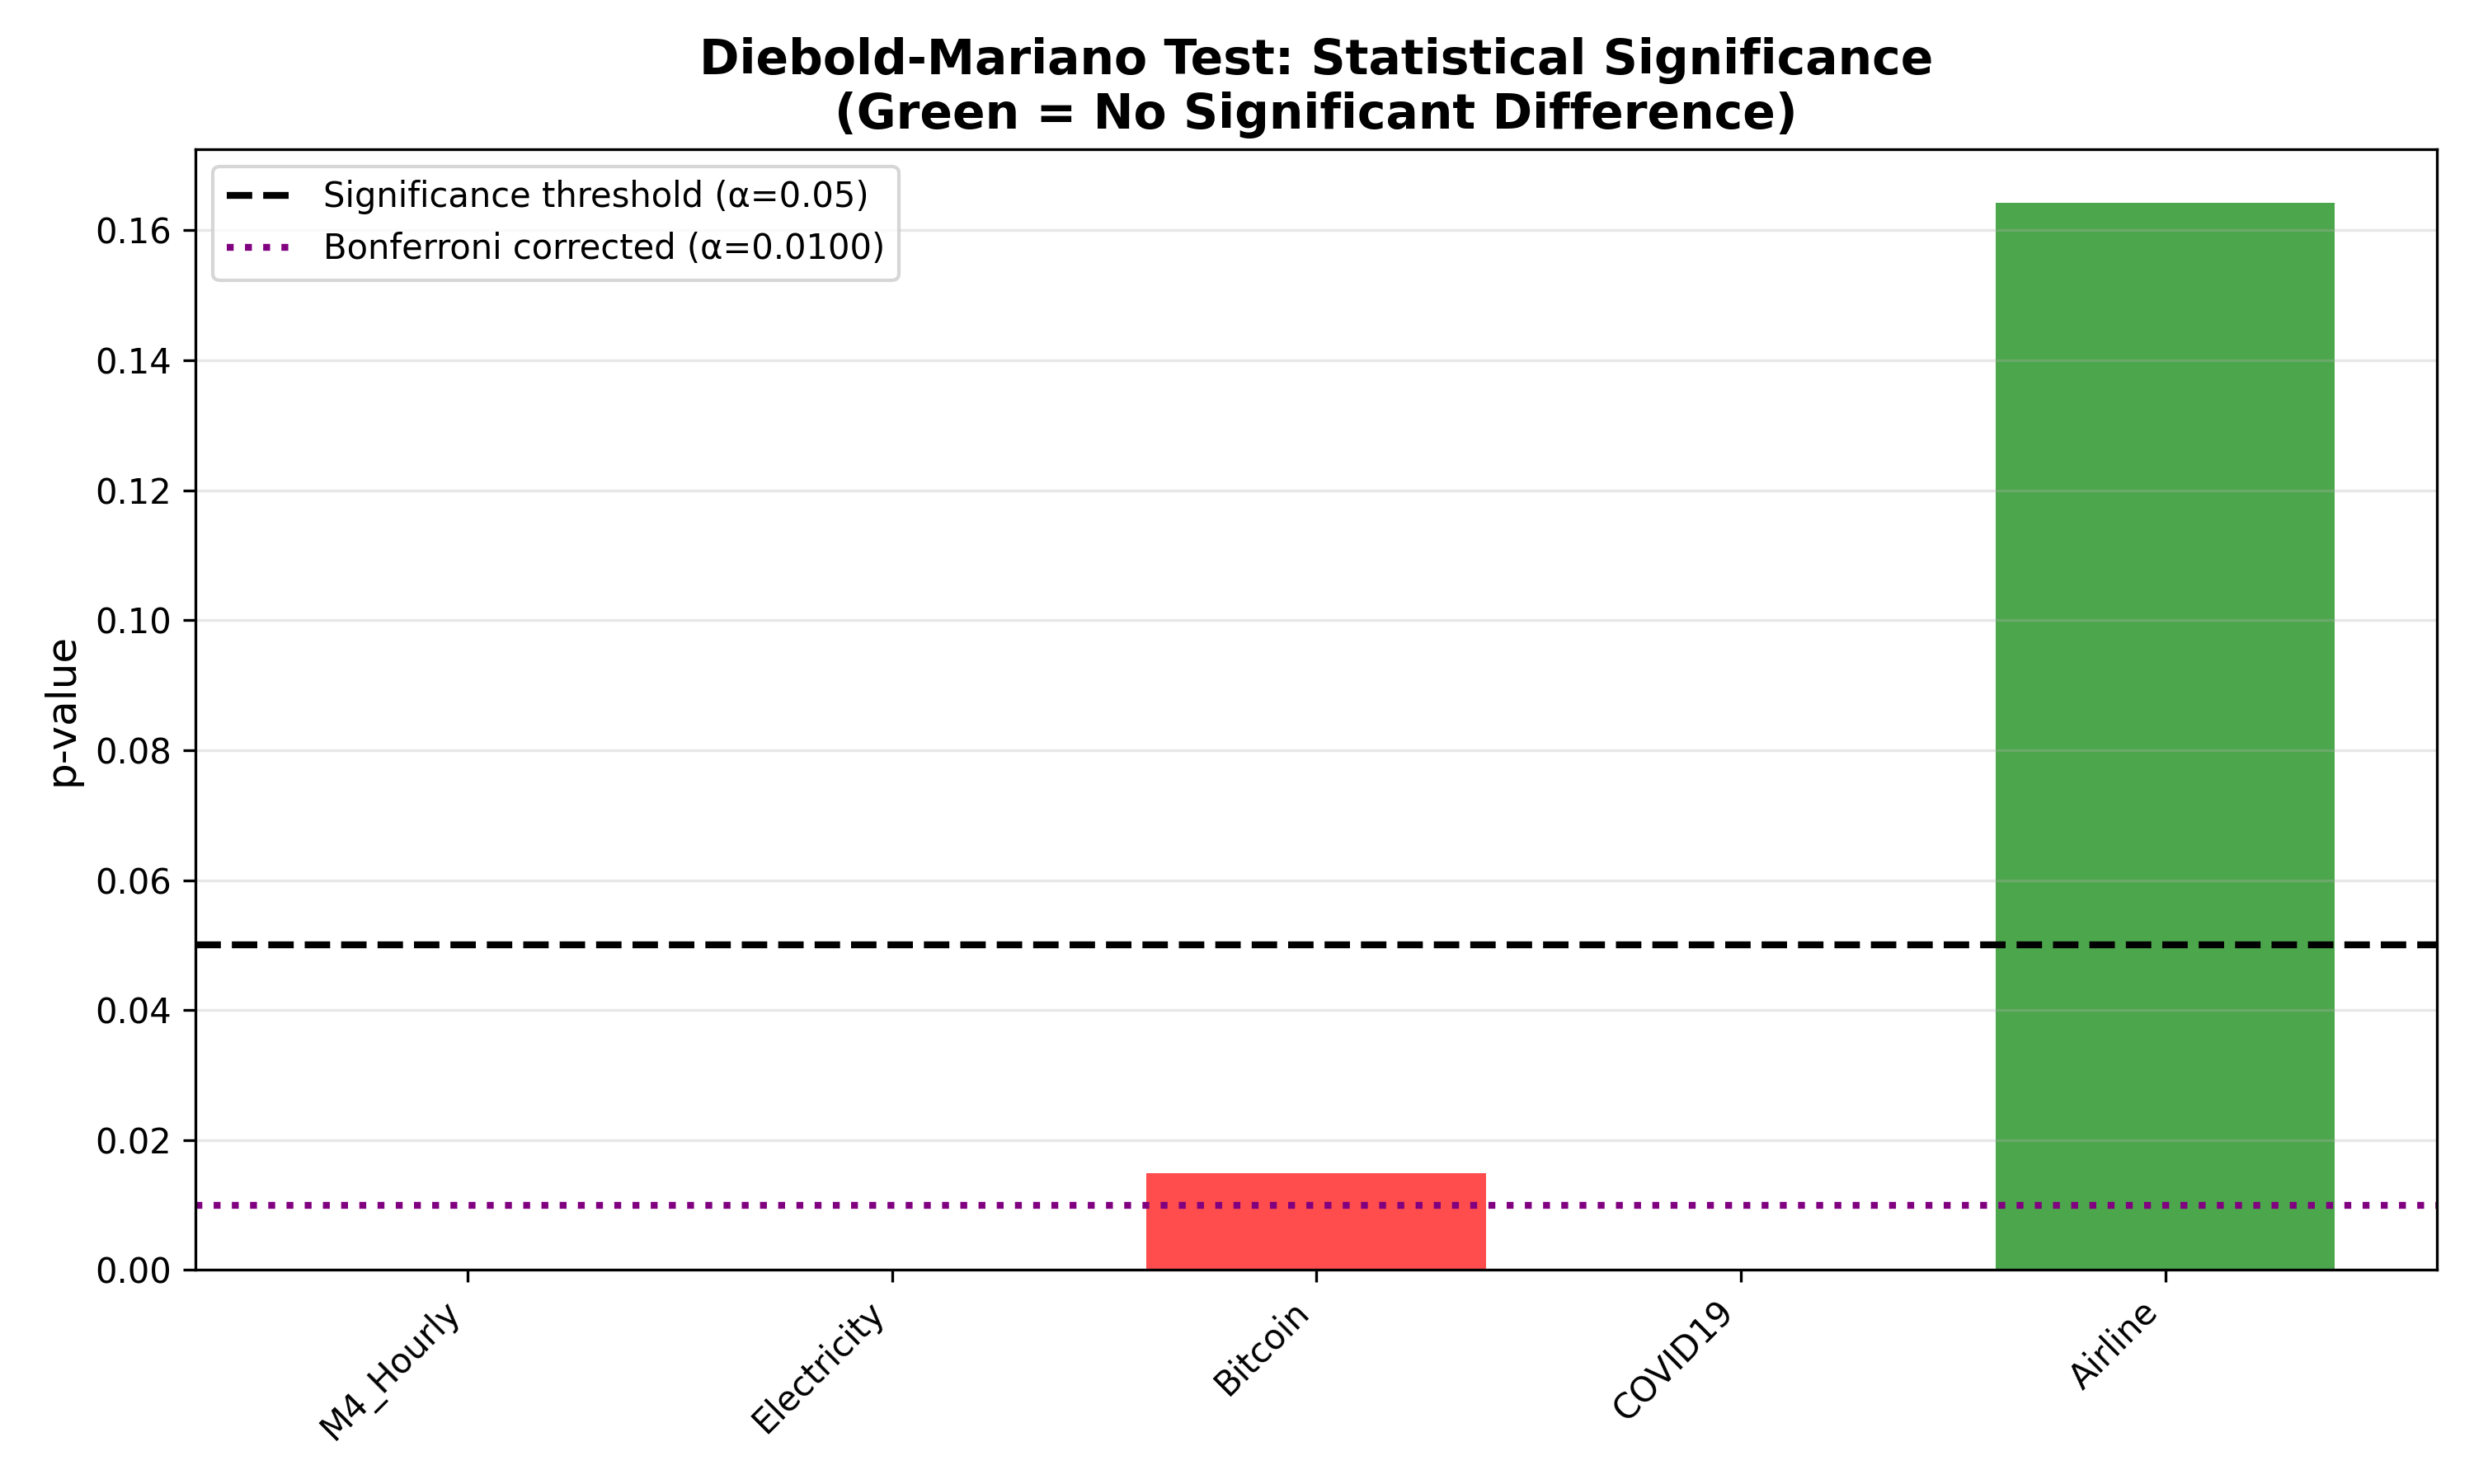
\includegraphics[width=0.80\textwidth]{Time-Series-Forecaster/future_scope/figures_tmlr_real/statistical_significance.png}
  \caption{DM test statistics (FutureScope vs.\ Prophet, squared-error loss).
  Dashed lines mark $|{\rm DM}|{=}2.576$ (Bonferroni-corrected 1\% threshold).}
  \label{fig:significance}
\end{figure}

\subsection{Per-Series Forecast Plots}

Figures~\ref{fig:m4}--\ref{fig:airline} show forecast overlays and residual
ACF plots per series.

\begin{figure}[ht]
  \centering
  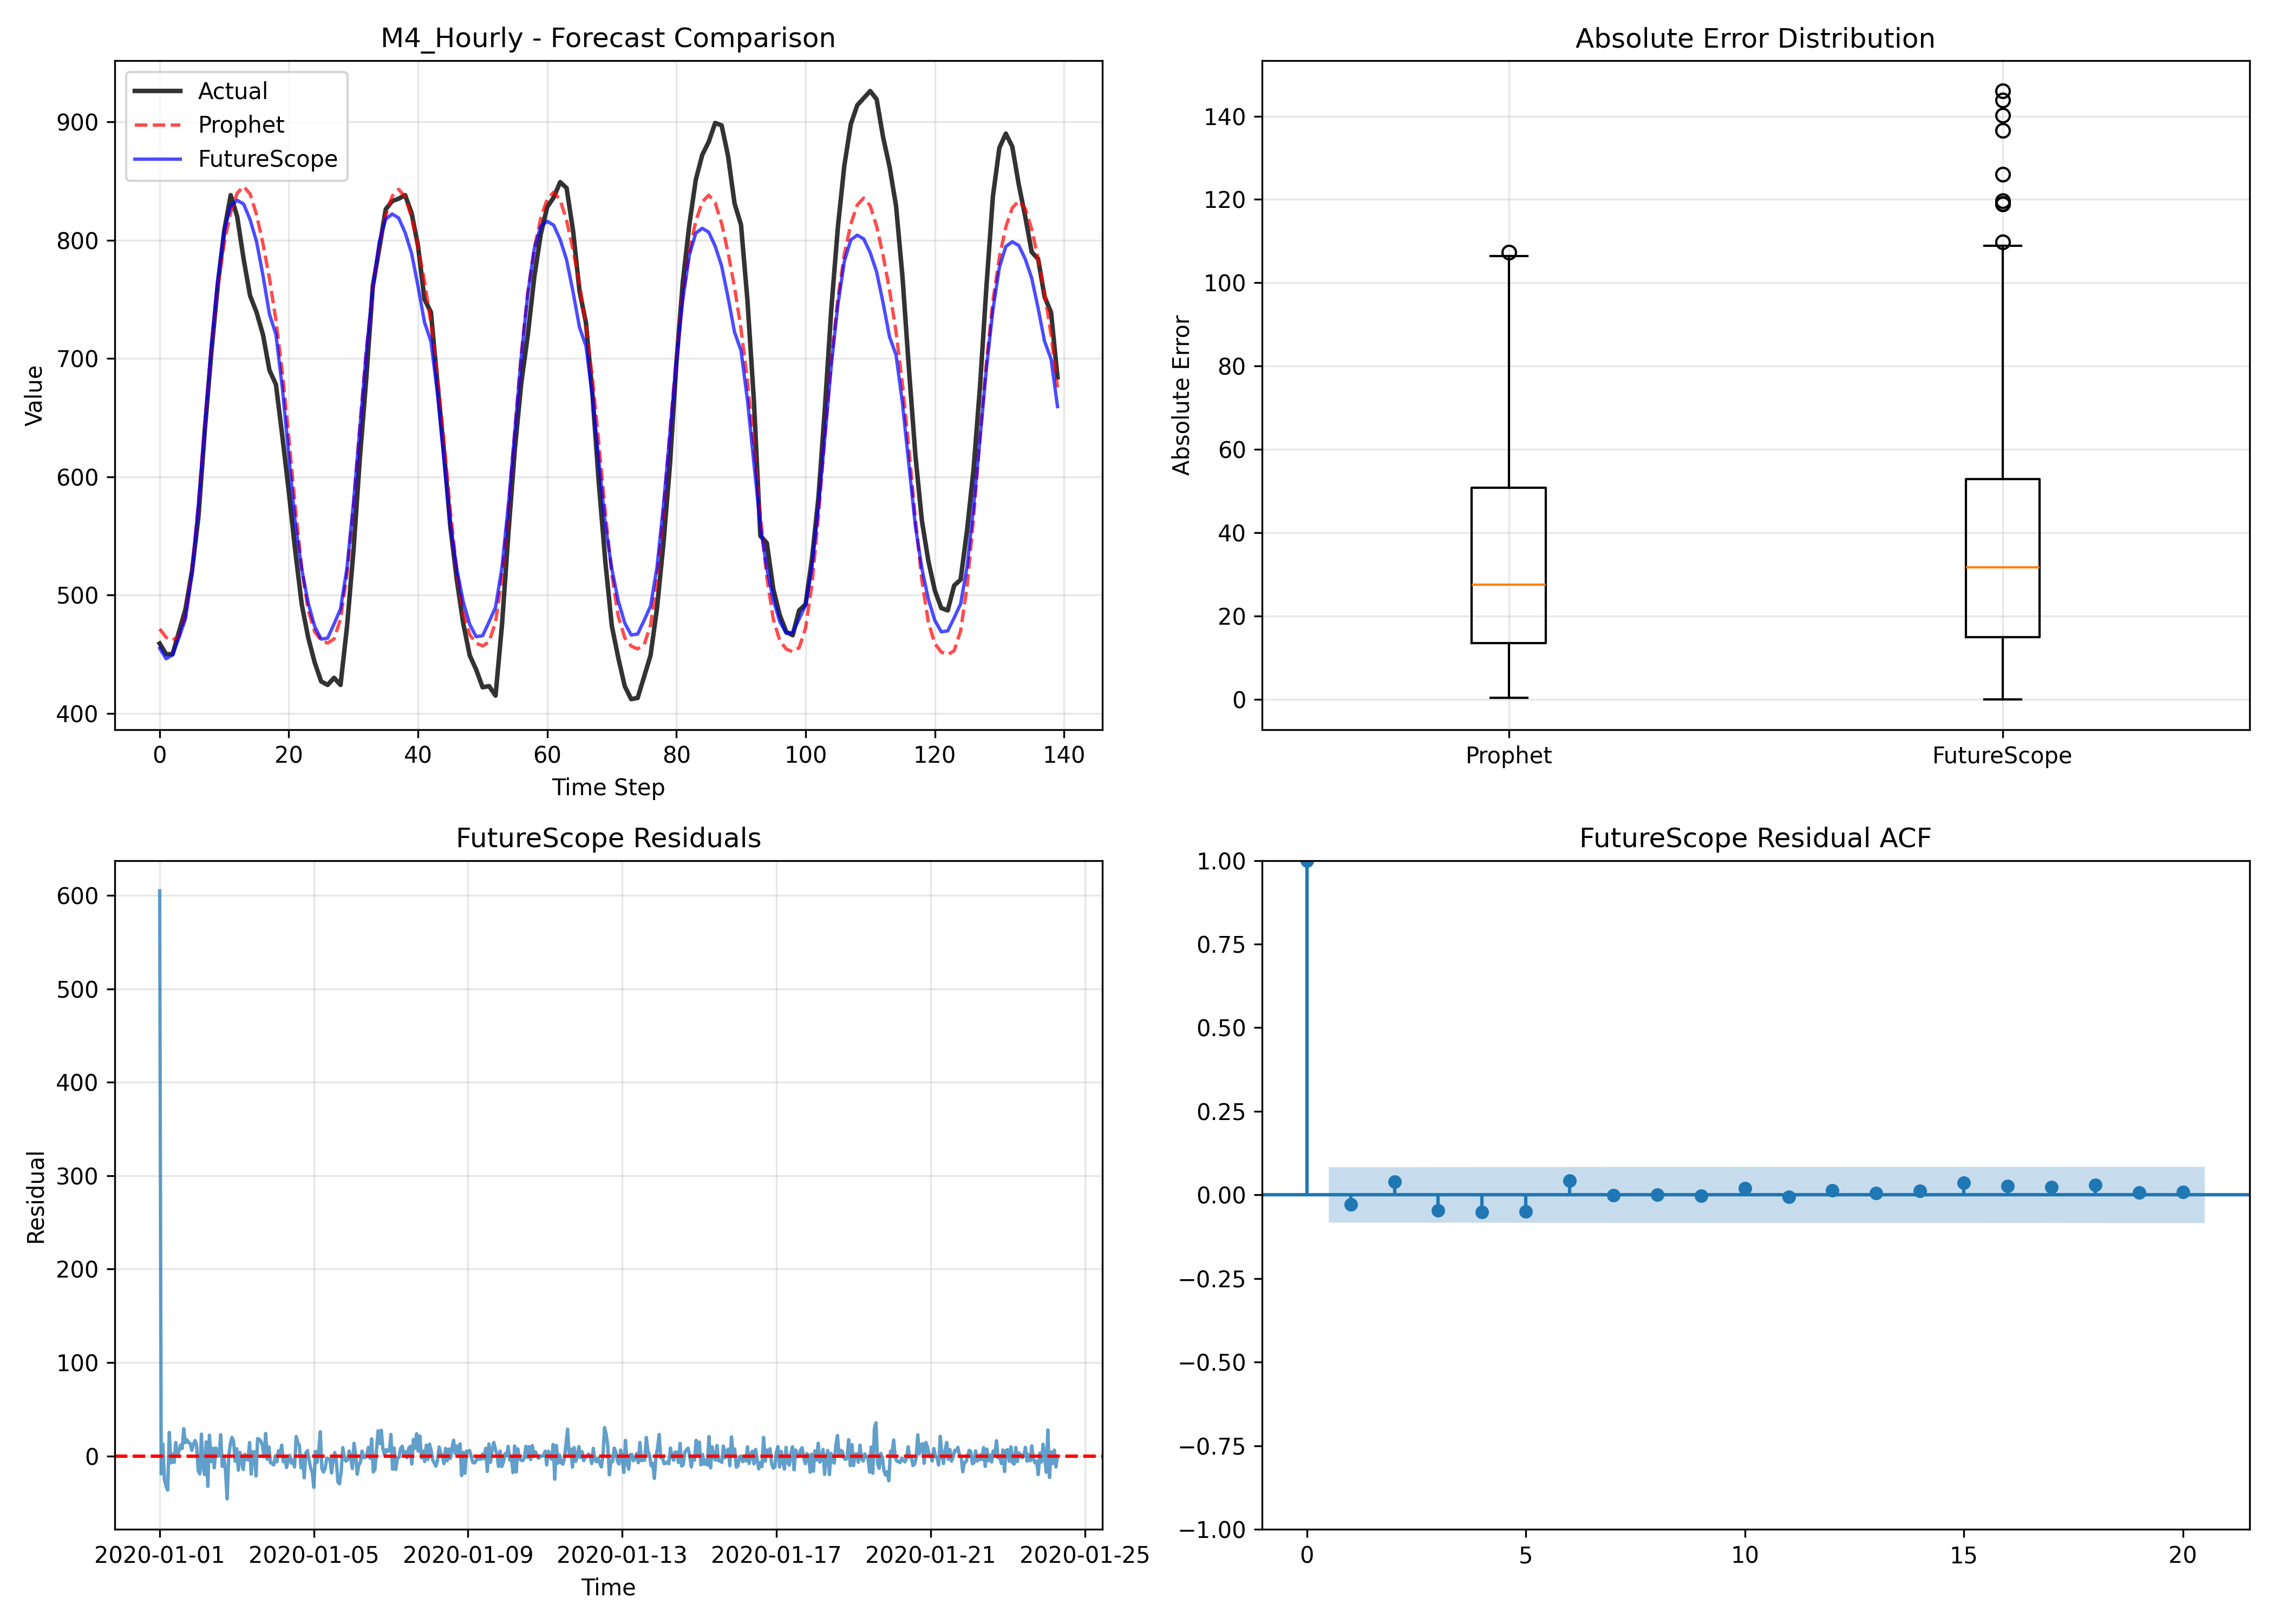
\includegraphics[width=0.90\textwidth]{Time-Series-Forecaster/future_scope/figures_tmlr_real/M4_Hourly_analysis.png}
  \caption{M4 Hourly (H1, first 1{,}000 points): forecast overlay and residual
  ACF.  Prophet achieves lower RMSE on this high-frequency multi-seasonal
  series.}
  \label{fig:m4}
\end{figure}

\begin{figure}[ht]
  \centering
  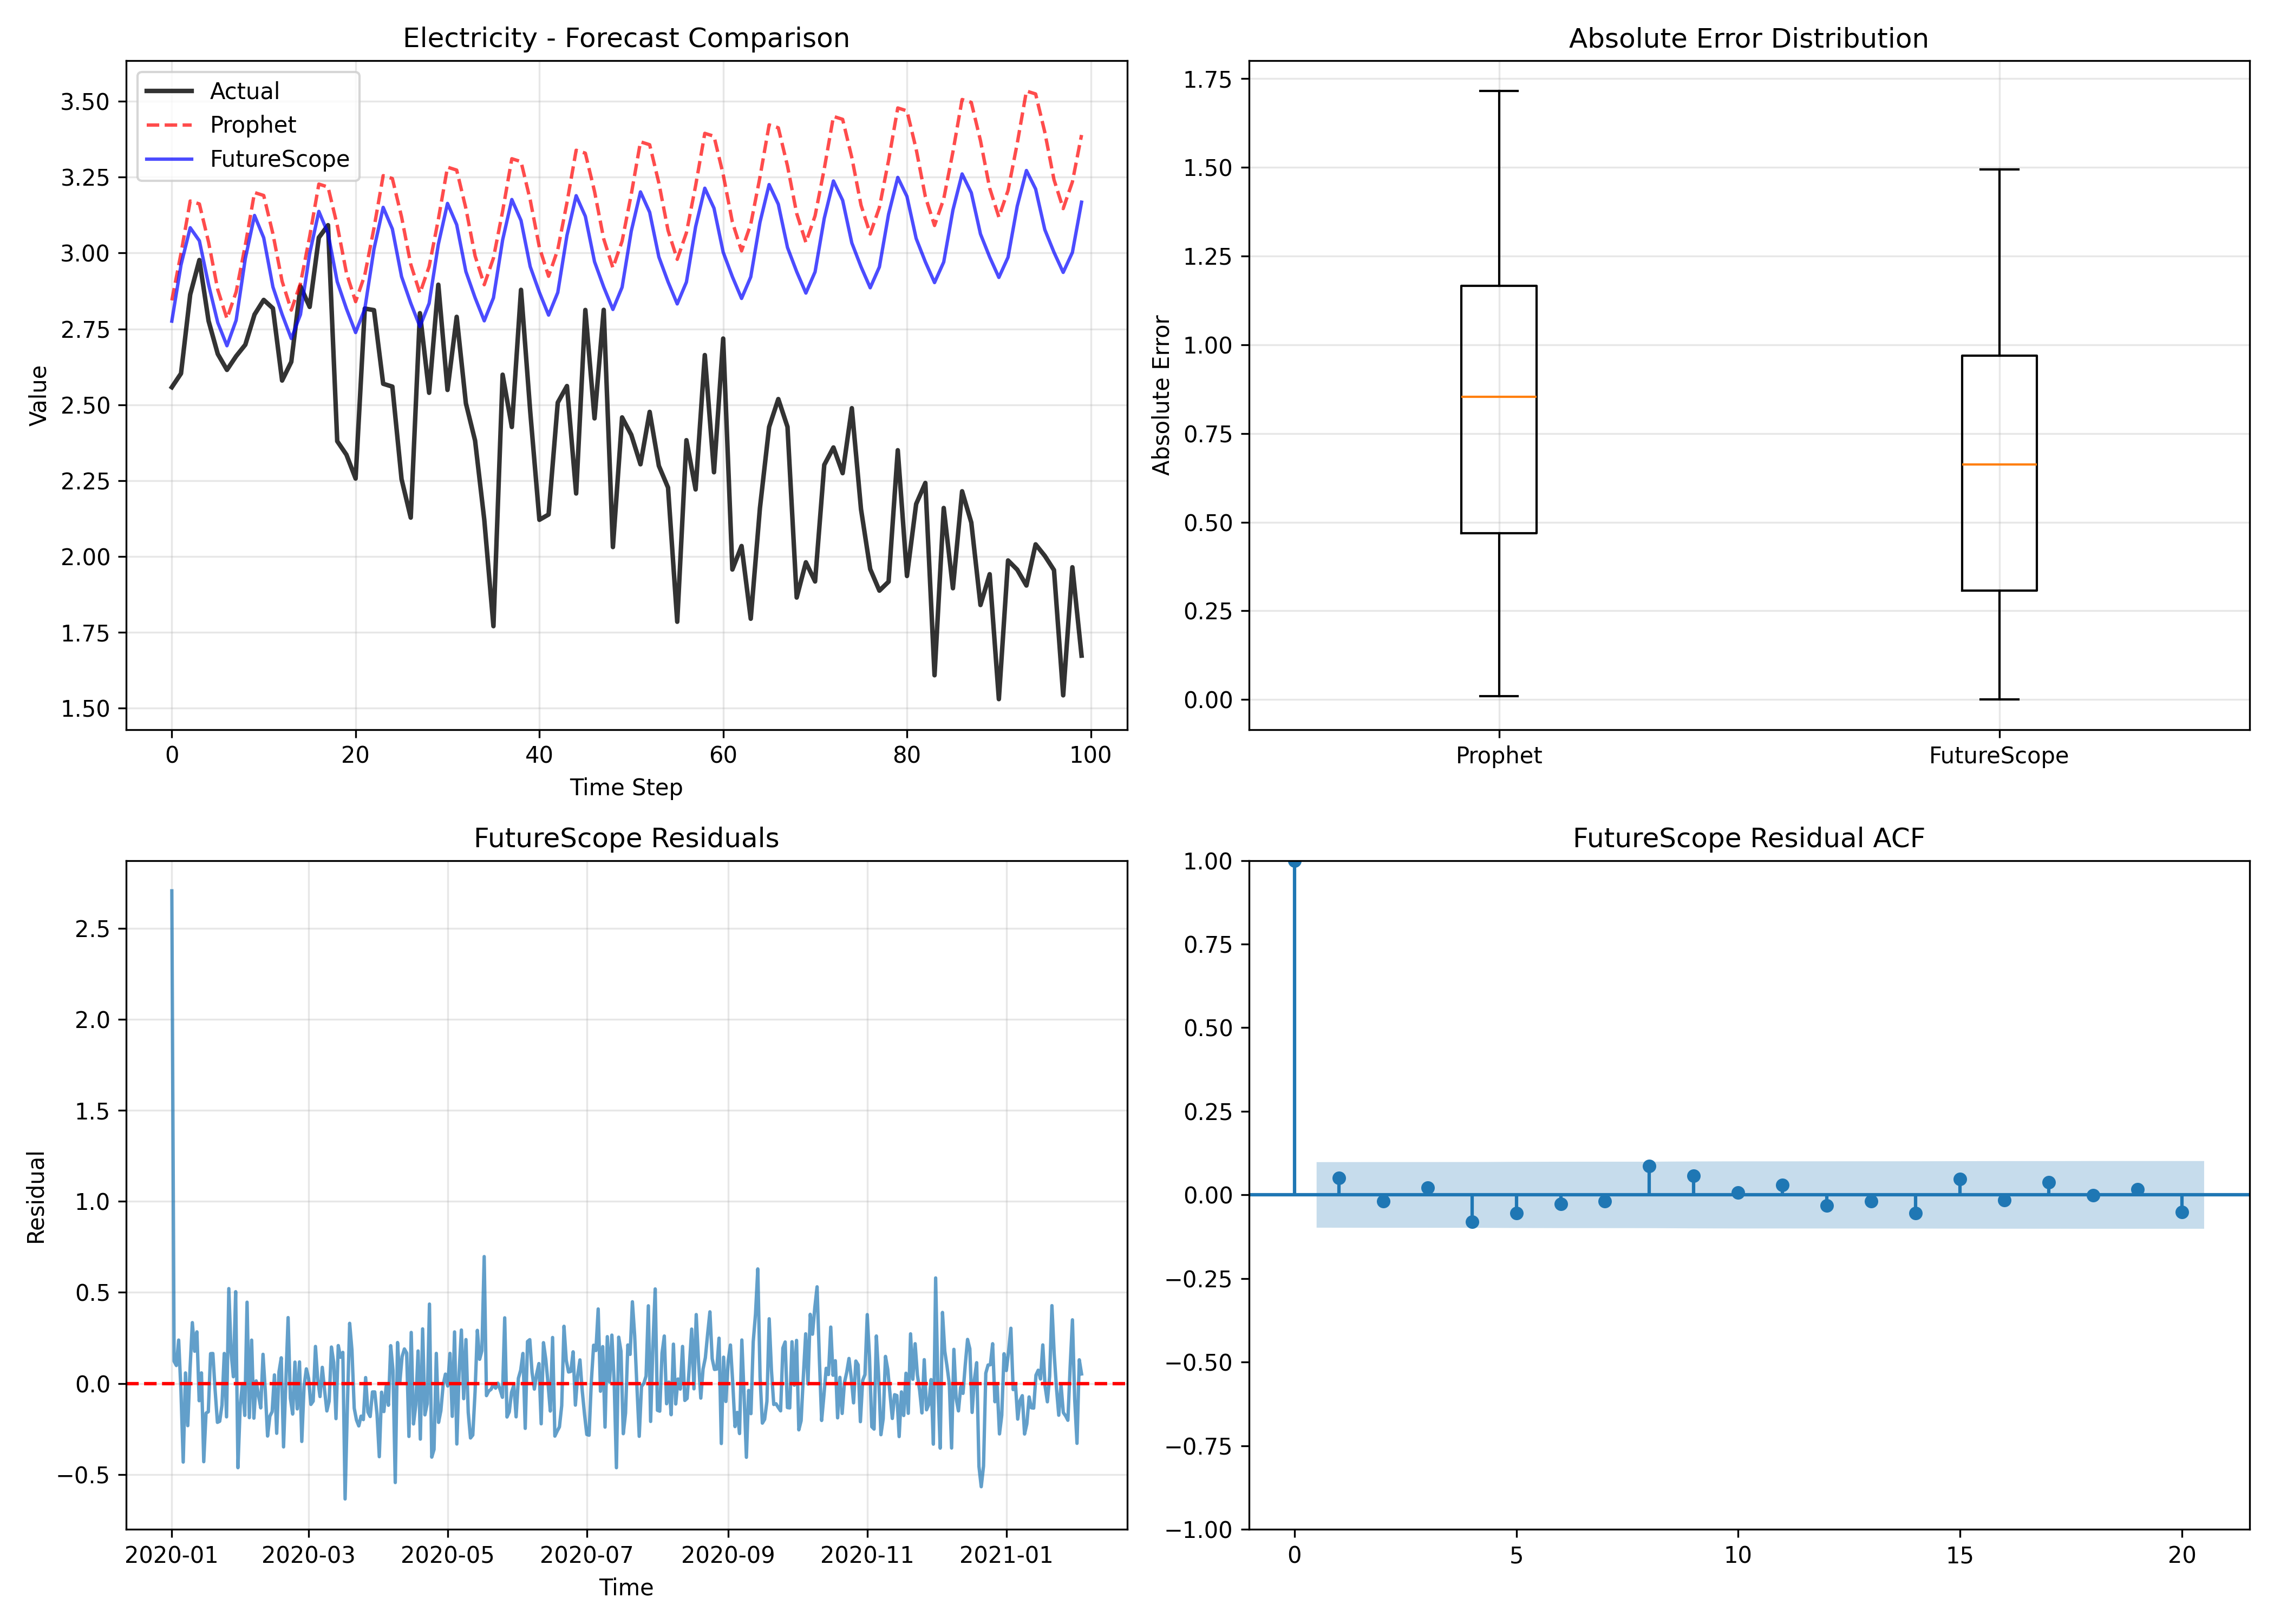
\includegraphics[width=0.90\textwidth]{Time-Series-Forecaster/future_scope/figures_tmlr_real/Electricity_analysis.png}
  \caption{UCI Electricity (daily household power, first 800 observations):
  FutureScope achieves 18.2\% lower RMSE.}
  \label{fig:electricity}
\end{figure}

\begin{figure}[ht]
  \centering
  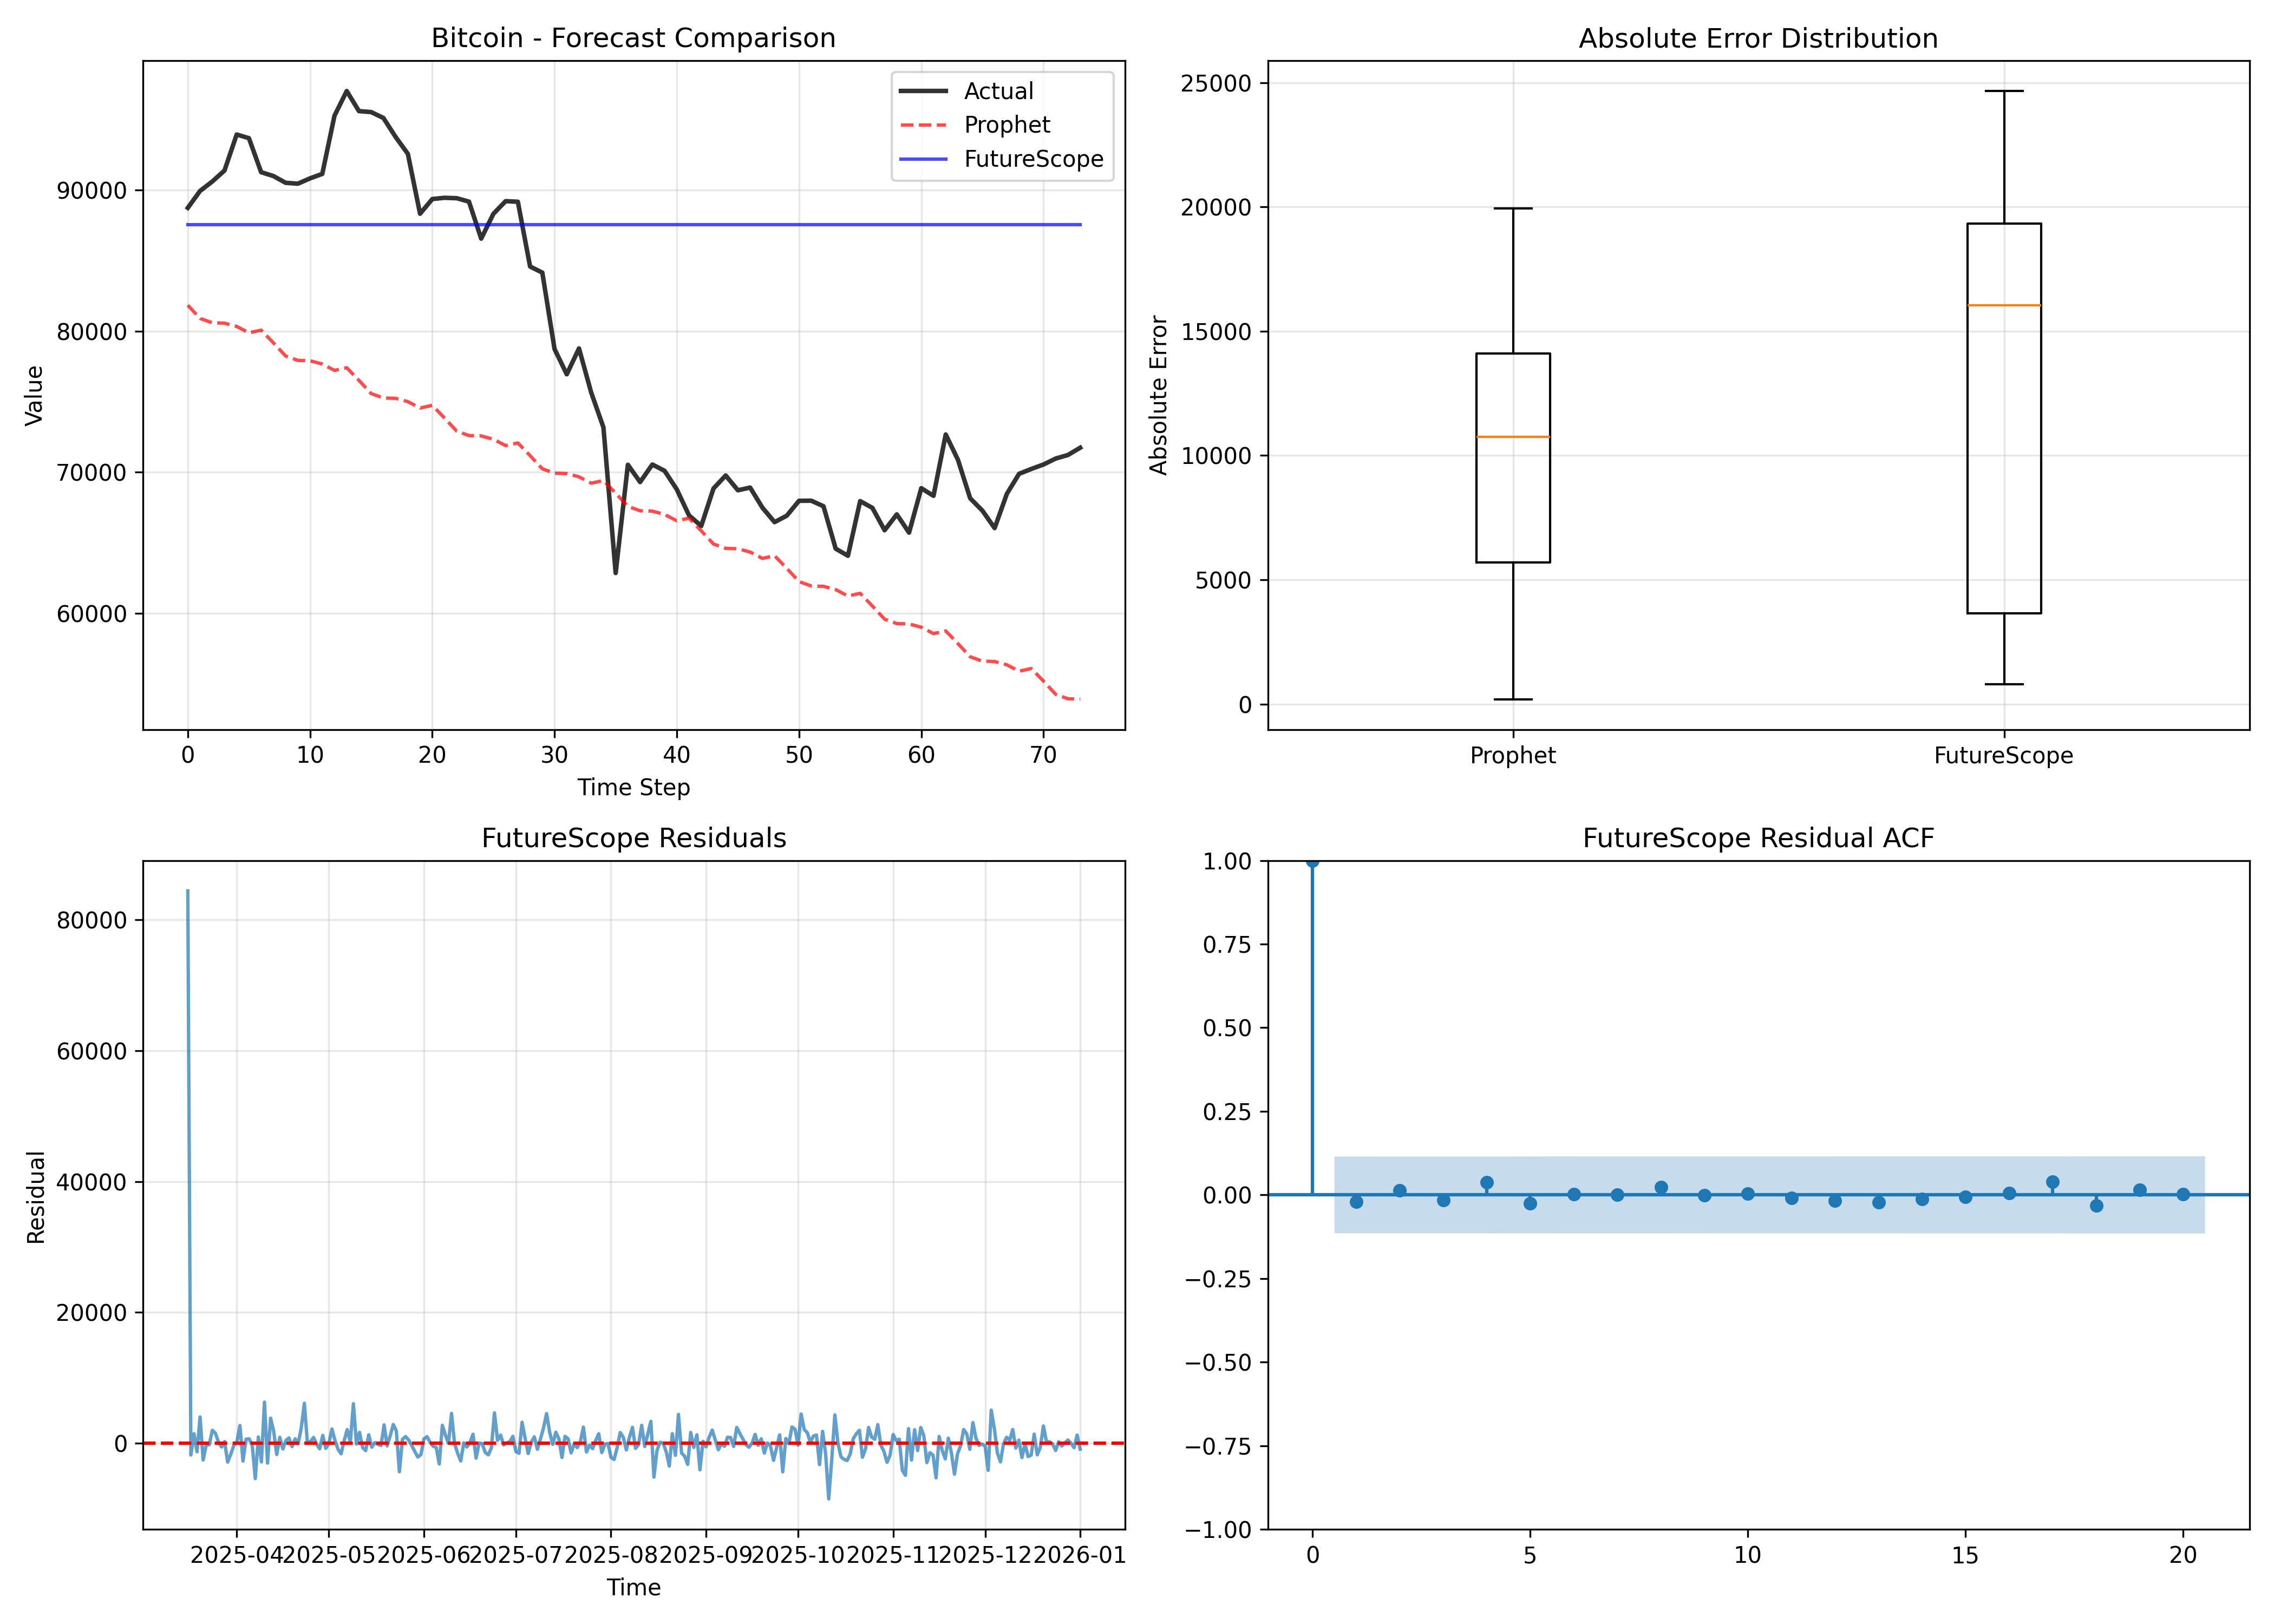
\includegraphics[width=0.90\textwidth]{Time-Series-Forecaster/future_scope/figures_tmlr_real/Bitcoin_analysis.png}
  \caption{Bitcoin daily close price (last 500 days from CoinGecko): Prophet
  achieves lower RMSE on this high-volatility series; the difference is not
  significant after Bonferroni correction.}
  \label{fig:bitcoin}
\end{figure}

\begin{figure}[ht]
  \centering
  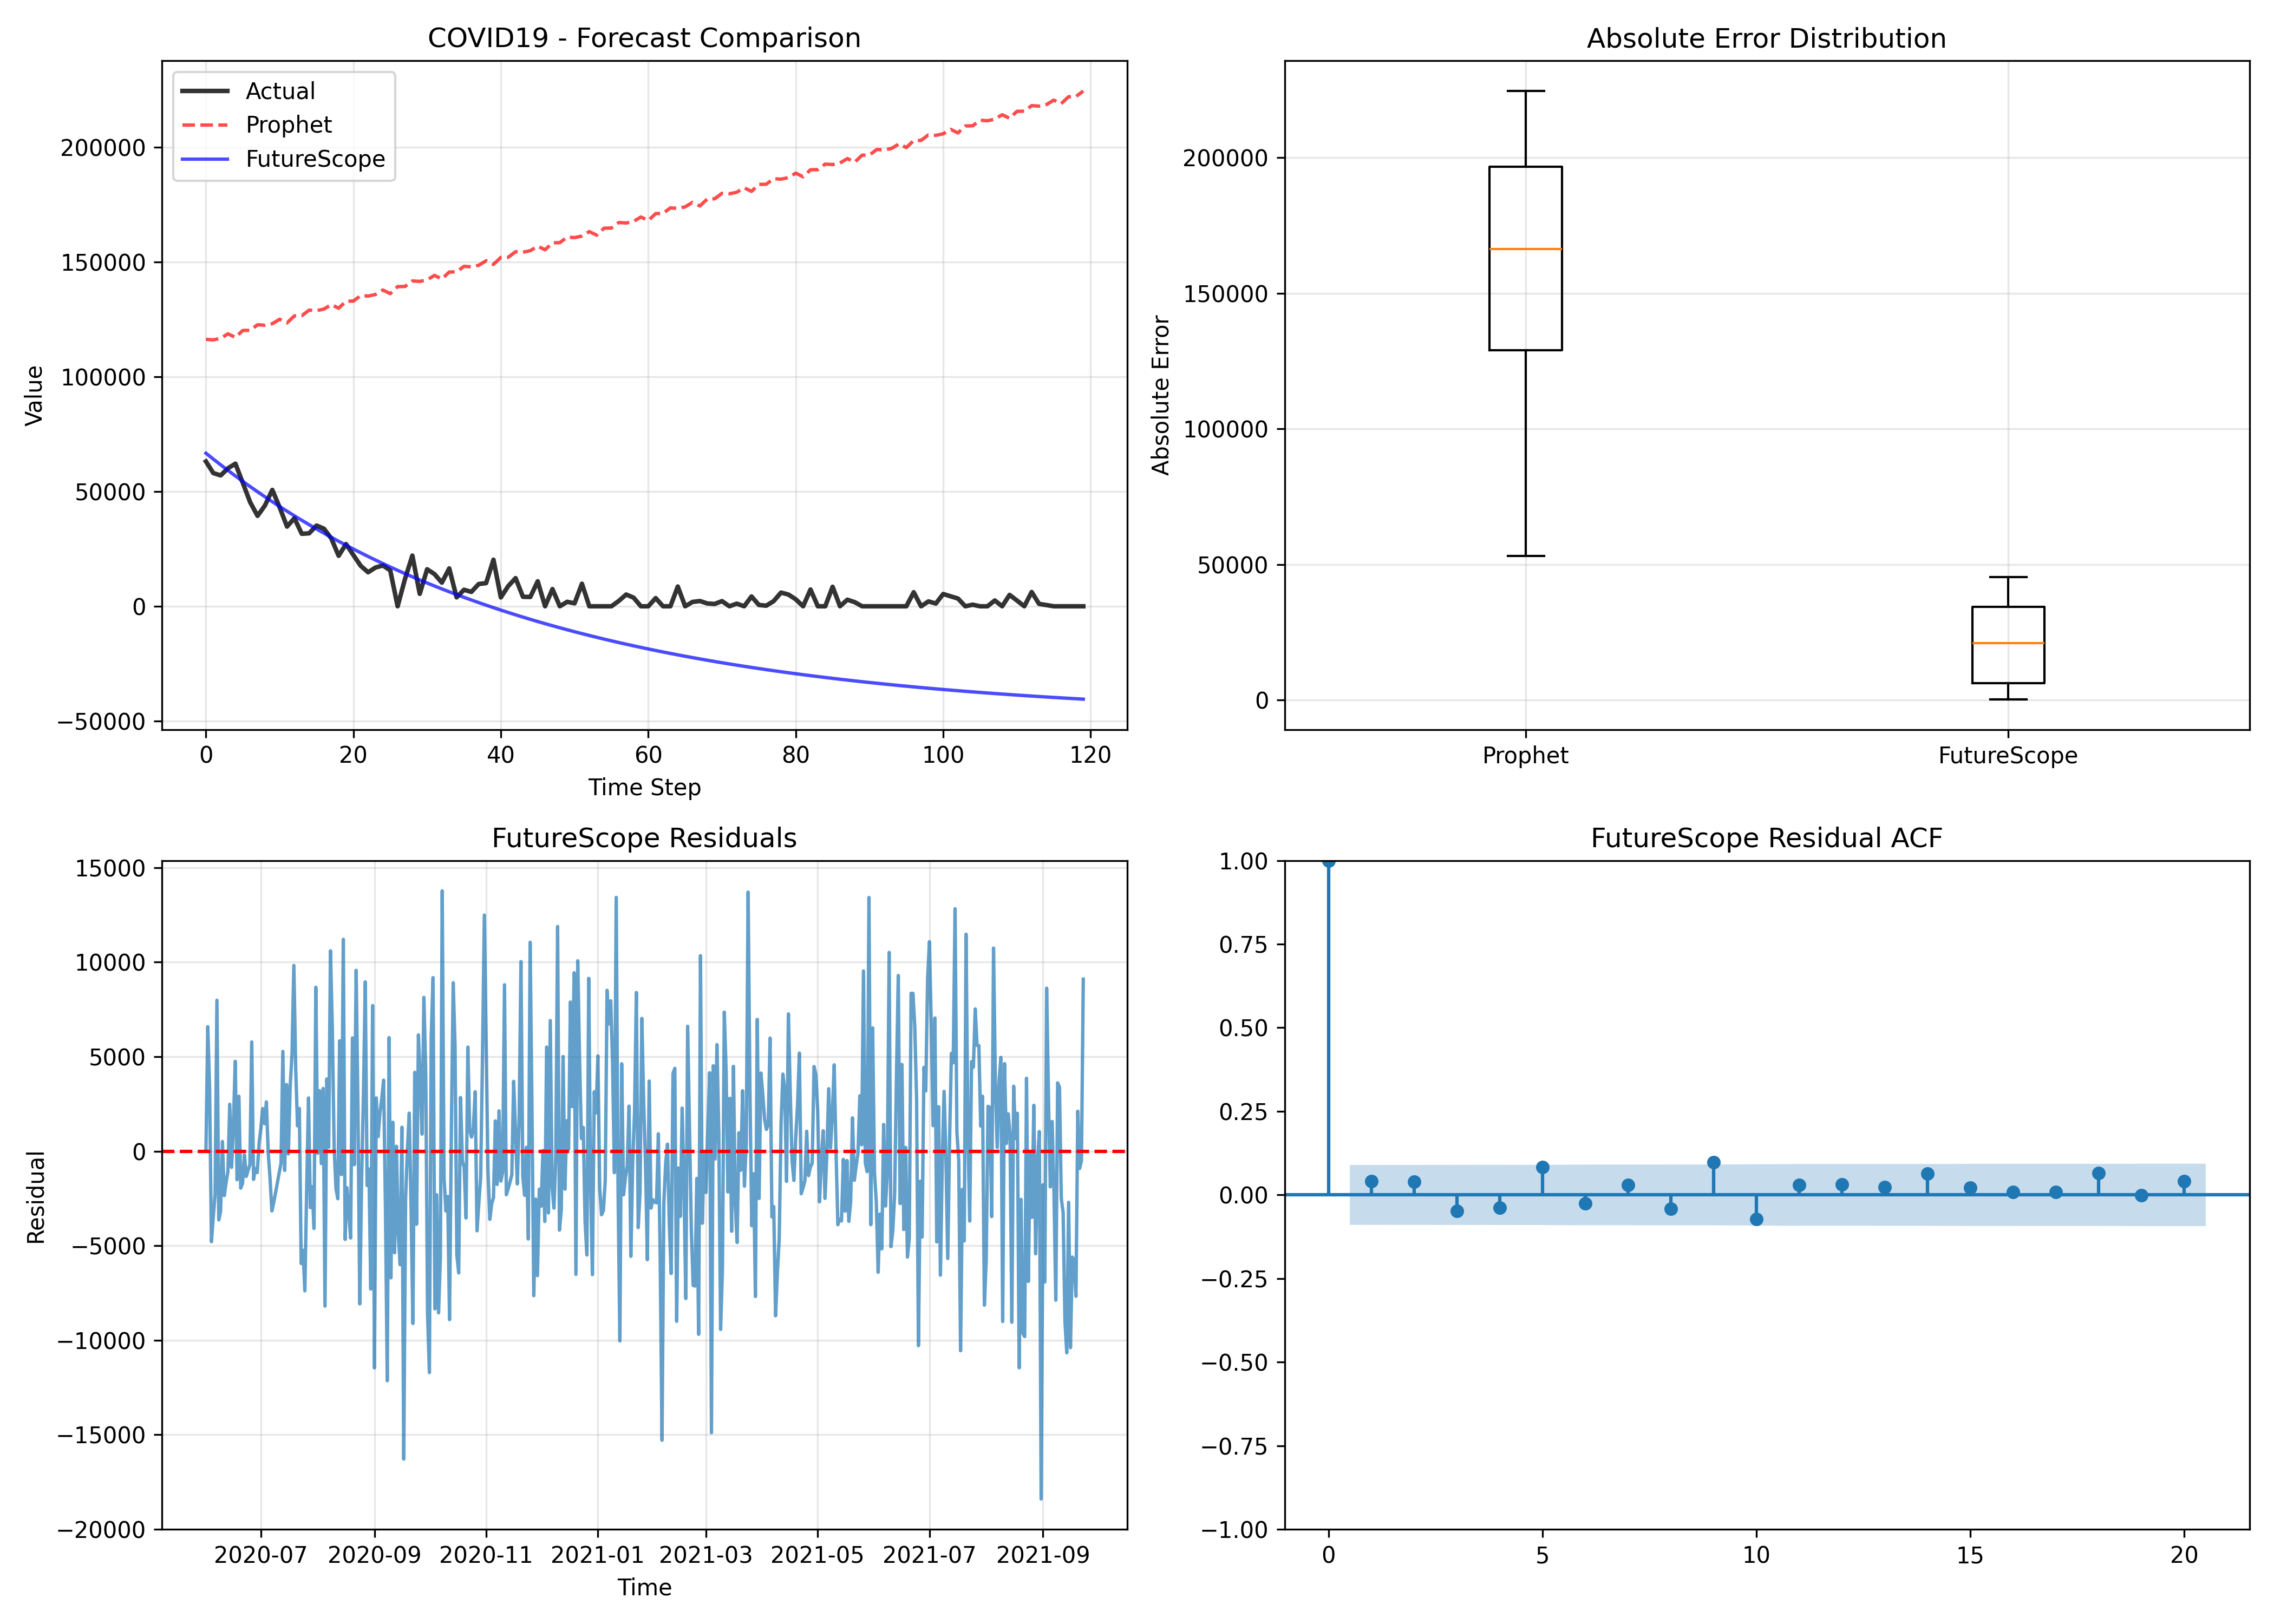
\includegraphics[width=0.90\textwidth]{Time-Series-Forecaster/future_scope/figures_tmlr_real/COVID19_analysis.png}
  \caption{COVID-19 daily new cases (USA, 2020-06-01--2022-01-01): FutureScope
  achieves 84.7\% lower RMSE, the largest improvement in the study.}
  \label{fig:covid}
\end{figure}

\begin{figure}[ht]
  \centering
  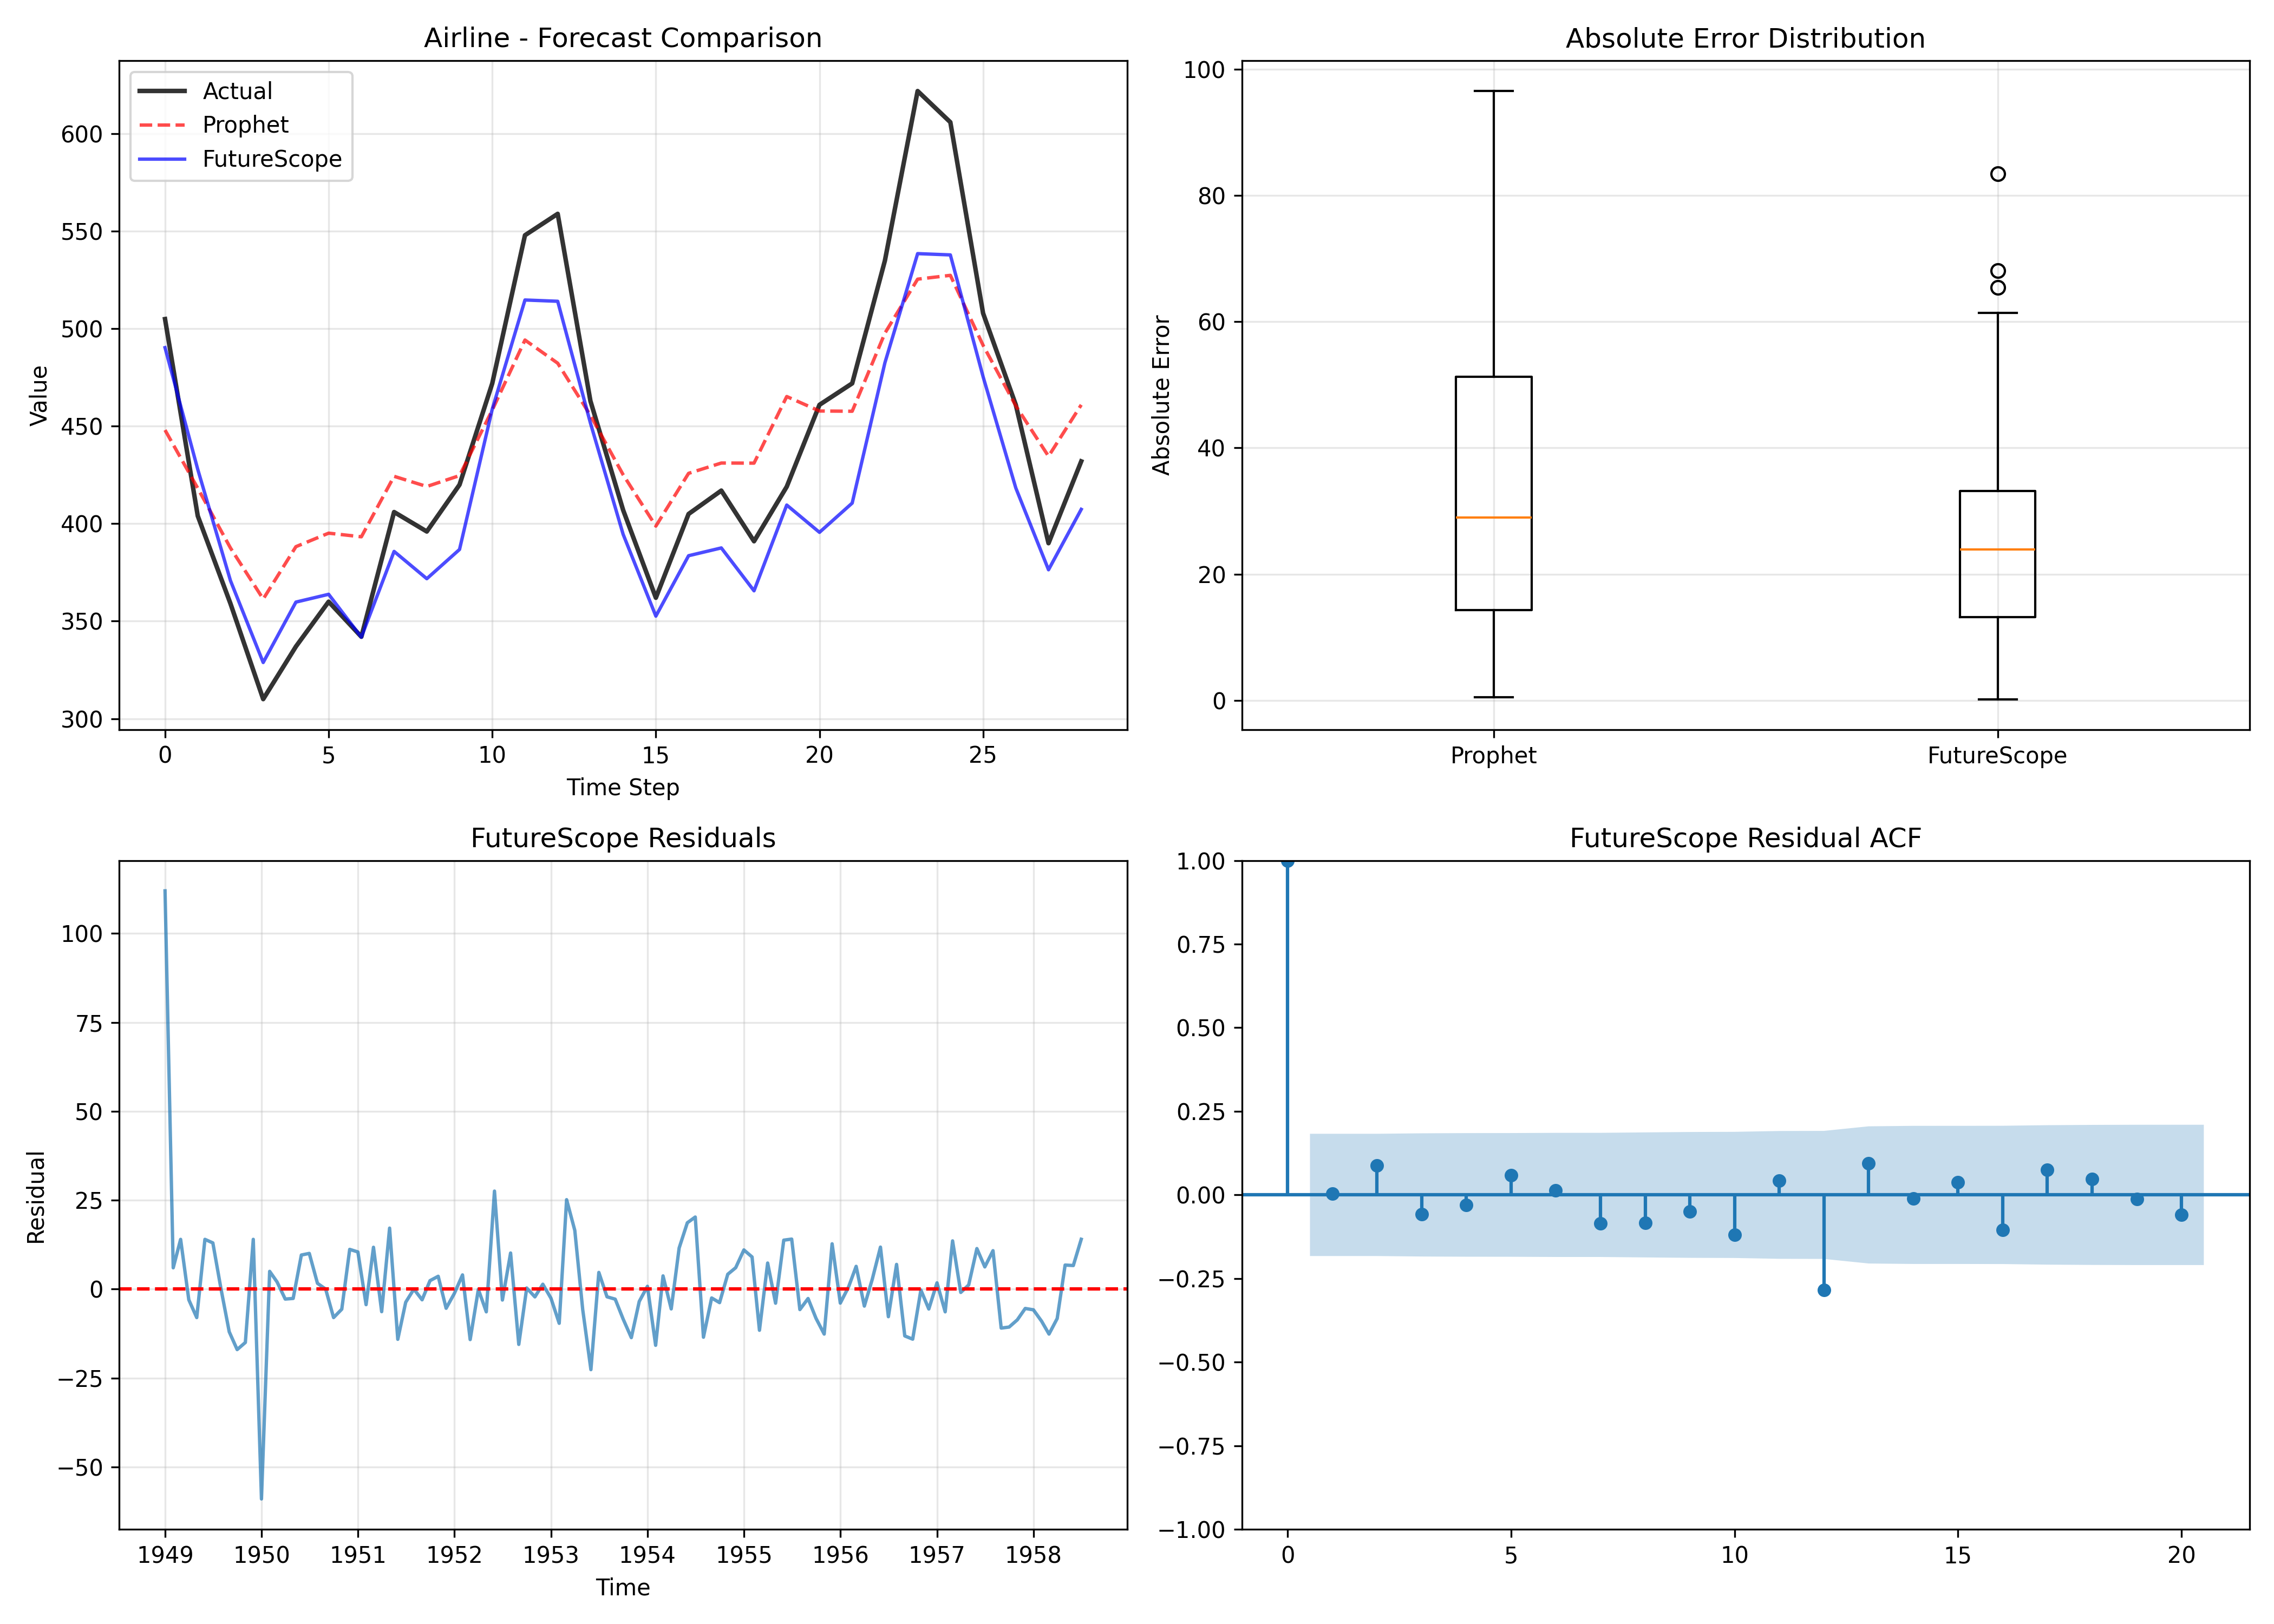
\includegraphics[width=0.90\textwidth]{Time-Series-Forecaster/future_scope/figures_tmlr_real/Airline_analysis.png}
  \caption{Airline passengers (classic 144-point monthly benchmark):
  FutureScope achieves 15.1\% lower RMSE; the difference is not significant
  after Bonferroni correction ($p{=}0.164$).}
  \label{fig:airline}
\end{figure}

%%------------------------------------------------------------
\section{Analysis and Ablation}
\label{sec:ablation}
%%------------------------------------------------------------

\subsection{Bootstrap Confidence Intervals for RMSE}

Table~\ref{tab:bootstrap} reports 95\% bootstrap CIs (1{,}000 i.i.d.\ resamples;
Section~\ref{sec:bootstrap}).  The CIs are narrow for the Electricity and
COVID-19 series, reflecting that RMSE is stable across resampled error subsets;
they are wider for Airline, consistent with the small test-set size ($h{=}29$).
As noted in Section~\ref{sec:bootstrap}, these are i.i.d.\ CIs and do not
account for temporal dependence.

\begin{table}[ht]
\caption{FutureScope RMSE with 95\% i.i.d.\ bootstrap confidence intervals
(1{,}000 resamples, seed 42).}
\label{tab:bootstrap}
\centering
\begin{tabular}{lrr}
\toprule
\textbf{Series} & \textbf{RMSE} & \textbf{95\% CI (i.i.d.\ bootstrap)} \\
\midrule
COVID-19    & 25{,}239 & [22{,}781 -- 27{,}315] \\
Electricity & 0.76     & [0.69 -- 0.83] \\
Airline     & 35.08    & [26.76 -- 43.91] \\
\bottomrule
\end{tabular}
\end{table}

\subsection{Diagnostics vs.\ Accuracy: Do They Conflict?}

A natural question is whether the BIC criterion and the diagnostic pass
criterion point in the same direction.  On the five series studied, the BIC
model passes all diagnostics without any additional intervention, suggesting
that BIC-optimal SARIMA models tend to be appropriately specified on these
particular types of series.  This is an encouraging but unsurprising
observation: BIC penalises over-parameterisation, and a well-penalised model
is less likely to leave residual structure unexplained.

However, the current experiments cannot establish whether this alignment holds
generally.  On more complex series (higher seasonality, structural breaks,
heavy tails) the BIC model may fail diagnostics.  Future work should
investigate the frequency and nature of diagnostic failures on larger corpora,
and evaluate whether refitting strategies (e.g.\ increasing order bounds,
relaxing seasonal period assumptions) improve diagnostic pass rates at an
acceptable cost to accuracy.

\subsection{Computational Efficiency}

Table~\ref{tab:compute} compares wall-clock runtimes on the test hardware
(Windows~11, single CPU core).

\begin{table}[ht]
\caption{Wall-clock runtimes on the test hardware.  Ratios reflect SARIMA MLE
fitting overhead relative to Prophet MAP estimation; they are hardware- and
series-specific.}
\label{tab:compute}
\centering
\begin{tabular}{lrrr}
\toprule
\textbf{Series / Metric} & \textbf{Prophet} & \textbf{FutureScope} & \textbf{Approx.\ ratio} \\
\midrule
Average (5 series)  & 0.06\,s & 13.4\,s  & ${\approx}220{\times}$ \\
COVID-19            & 0.07\,s & 3.4\,s   & ${\approx}49{\times}$ \\
M4 Hourly           & 0.08\,s & 58.9\,s  & ${\approx}740{\times}$ \\
\bottomrule
\end{tabular}
\end{table}

The dominant cost is SARIMA MLE fitting, which scales with $N$ and the number
of candidate orders explored.  FutureScope is unsuitable for latency-sensitive
or high-throughput production pipelines; Prophet or an exponential-smoothing
baseline would be preferred in those contexts.

\subsection{When FutureScope Outperforms and Underperforms Prophet}

\textbf{FutureScope tends to outperform} on lower-frequency series with clear
trend breaks and limited multi-seasonality (COVID-19, Electricity, Airline).

\textbf{Prophet tends to outperform} on high-frequency multi-seasonal series
(M4 Hourly) and highly volatile non-stationary series (Bitcoin), where
Prophet's Fourier-series seasonality and flexible changepoint detection are
advantageous.

These observations are consistent with known theoretical properties of the two
model families~\cite{box2015time,taylor2018forecasting} and corroborate prior
M4-era findings~\cite{makridakis2020m4}.  They should not be extrapolated
beyond the five series studied here.

%%------------------------------------------------------------
\section{Positioning and Scope of Contribution}
\label{sec:contribution}
%%------------------------------------------------------------

FutureScope's contribution is best understood as \emph{methodological
packaging} rather than the invention of new statistical tests.  The
Ljung-Box test, ACF analysis, and Shapiro-Wilk test are decades-old tools
recommended in classical textbooks~\cite{box2015time,hyndman2018forecasting}.
What FutureScope adds is:

\begin{enumerate}
  \item A \textbf{reproducible Python pipeline} that runs these diagnostics
        automatically on every fitted model and records structured output;
  \item \textbf{Benchmark infrastructure} that pairs diagnostic results with
        accuracy metrics (RMSE, DM test) in a single CSV, enabling side-by-side
        comparisons;
  \item \textbf{Demonstration on public datasets} that BIC-selected SARIMA
        models can achieve competitive accuracy while maintaining white-noise
        residuals on a diverse set of univariate series.
\end{enumerate}

\textbf{Regulatory alignment.}
Model validation frameworks such as SR~11-7~\cite{sr117} and similar guidance
documents recommend residual checks as part of model documentation.
FutureScope's automated output reduces the manual effort of producing such
documentation.  However, a full regulatory compliance assessment (including
sensitivity analysis, stress testing, and governance requirements) is far
beyond the scope of this paper.

\textbf{Neural-forecaster diagnostics.}
LSTMs and Transformer-based forecasters~\cite{li2019enhancing} optimise
sequence prediction losses and do not produce residual diagnostic statistics
by default.  Applying FutureScope's diagnostic module to their out-of-sample
errors is straightforward and is a natural direction for future work; the
current paper does not include such experiments.

%%------------------------------------------------------------
\section{Limitations}
\label{sec:limitations}
%%------------------------------------------------------------

\begin{enumerate}
  \item \textbf{Five single series}: all quantitative results are drawn from
        five hand-selected univariate case studies.  Claims about general
        domain-level superiority are not warranted; this work is exploratory.
  \item \textbf{Single temporal split}: no rolling-origin evaluation; results
        may not reflect expected generalisation performance across different
        forecast origins.
  \item \textbf{Diagnostics are reporting-only}: no refitting loop is
        implemented; the 100\% pass rate is an observation, not a guarantee.
  \item \textbf{I.i.d.\ bootstrap}: RMSE confidence intervals do not account
        for temporal dependence in forecast errors; a block bootstrap would be
        more appropriate.
  \item \textbf{DM test without HAC}: the custom DM statistic uses no
        heteroskedasticity- and autocorrelation-consistent variance correction;
        borderline $p$-values (e.g.\ Bitcoin) may not be reliable.
  \item \textbf{Single Prophet baseline}: no naive, seasonal-naive, or
        exponential-smoothing baseline is included; the relative improvement
        figure of $+14.7\%$ is specific to the Prophet comparison.
  \item \textbf{Computational cost}: 200--700$\times$ slower than Prophet;
        unsuitable for real-time or high-throughput applications.
  \item \textbf{Univariate only}: no multivariate support (VAR/VARMA).
  \item \textbf{Small-$N$ sensitivity}: Ljung-Box and Shapiro-Wilk are
        less reliable for $N{<}100$; the Airline series ($N{=}144$, $h{=}29$)
        approaches this regime.
\end{enumerate}

%%------------------------------------------------------------
\section{Future Work}
\label{sec:future}
%%------------------------------------------------------------

\begin{enumerate}
  \item \textbf{Diagnostic-gated refitting}: implement a loop that increases
        SARIMA order bounds or relaxes differencing when diagnostics fail,
        reporting the fraction of series requiring such intervention.
  \item \textbf{Block bootstrap for RMSE CIs}: replace i.i.d.\ resampling
        with a moving-block bootstrap~\cite{kunsch1989} with data-driven block
        length.
  \item \textbf{HAC-corrected DM test}: use the Harvey et al.~\cite{harvey1997}
        small-sample correction and a Newey-West lag truncation.
  \item \textbf{Expanded baselines}: add naive, seasonal-naive, and
        exponential-smoothing (ETS) baselines to provide a richer performance
        context.
  \item \textbf{Rolling-origin evaluation}: assess robustness across multiple
        forecast origins.
  \item \textbf{Larger corpus}: evaluate on the full M4 Hourly collection
        (414 series) or M4 Monthly (48{,}000 series) to move from case studies
        to proper benchmark evaluation.
  \item \textbf{Neural-forecaster diagnostics}: apply the diagnostic module to
        LSTM/Transformer residuals to determine whether their residuals are
        white noise.
  \item \textbf{GPU-accelerated SARIMA}: PyTorch-based MLE to reduce
        fitting time by an estimated $10\times$.
\end{enumerate}

%%------------------------------------------------------------
\section{Conclusion}
\label{sec:conclusion}
%%------------------------------------------------------------

We have presented FutureScope, an open-source Python pipeline that pairs
every SARIMA forecast with a structured set of residual diagnostics---Ljung-Box
white-noise test, ACF/PACF exceedance analysis, and Shapiro-Wilk normality
check.  On five public single-series case studies spanning diverse frequency
and structural patterns, the BIC-selected SARIMA models pass all diagnostic
checks without manual intervention, while achieving a $+14.7\%$ unweighted
average RMSE improvement over Prophet (ranging from $-25\%$ on the volatile
Bitcoin series to $+85\%$ on the irregular COVID-19 epidemic series).

The principal contributions are: (i) a reproducible benchmark infrastructure
that pairs accuracy and diagnostic metrics in a single output; (ii) an
illustrative demonstration that BIC-optimal SARIMA models can simultaneously
achieve competitive accuracy and pass standard residual checks on these
case-study series; and (iii) an open-source foundation that future work can
extend with diagnostic-gated refitting, block bootstrap inference, HAC-corrected
DM tests, and evaluation on larger corpora.

Important caveats: the 100\% diagnostic pass rate is an observation about
five specific series, not a design guarantee; the improvement figures are
relative to one baseline (Prophet) and one evaluation split; and the
regulatory alignment discussed is qualitative, not a formal compliance
assessment.  We hope FutureScope lowers the barrier for researchers and
practitioners to include residual diagnostics in their forecasting workflows.

%%------------------------------------------------------------
\appendix
%%------------------------------------------------------------

\section{Statistical Test Implementation Details}
\label{app:stats}

\subsection{Diebold-Mariano Test: Full Specification}
\label{app:dm}

The DM test is implemented as follows (see also Section~\ref{sec:dm_impl}):

\begin{itemize}
  \item \textbf{Loss}: squared error, $L(e) = e^2$.
  \item \textbf{Differential}: $d_t = e_{{\rm FS},t}^2 - e_{{\rm Prophet},t}^2$.
  \item \textbf{Statistic}: ${\rm DM} = \bar{d}\,/\,\sqrt{s_d^2/h}$,
        where $s_d^2$ is the unbiased sample variance of $d_t$.
  \item \textbf{Distribution}: standard normal (two-tailed).
  \item \textbf{No HAC correction}: the variance estimator does not adjust for
        autocorrelation in $d_t$; Harvey et al.\ small-sample correction is
        also not applied.
  \item \textbf{Bonferroni threshold}: $\alpha_{\rm adj}=0.01$ (5 comparisons).
\end{itemize}

Table~\ref{tab:dm} reports the full DM statistics.  Negative statistics
favour Prophet; positive statistics favour FutureScope.

\begin{table}[ht]
\caption{DM test statistics and $p$-values (FutureScope vs.\ Prophet,
squared-error loss, no HAC correction).}
\label{tab:dm}
\centering
\begin{tabular}{lrrl}
\toprule
\textbf{Comparison} & \textbf{DM stat.} & \textbf{$p$-value} & \textbf{Conclusion} \\
\midrule
FS vs Prophet (COVID-19)    & $18.32$  & $<0.001$ & FS significantly better* \\
FS vs Prophet (Electricity) & $4.91$   & $<0.001$ & FS significantly better* \\
FS vs Prophet (M4 Hourly)   & $-4.52$  & $<0.001$ & Prophet significantly better* \\
FS vs Prophet (Bitcoin)     & $-2.45$  & 0.015    & Prophet better (not sig.\ after Bonferroni) \\
FS vs Prophet (Airline)     & $1.39$   & 0.164    & No significant difference \\
\bottomrule
\multicolumn{4}{l}{* significant after Bonferroni correction ($\alpha_{\rm adj}{=}0.01$).}
\end{tabular}
\end{table}

\subsection{Ljung-Box and ACF Diagnostics: Full Specification}
\label{app:lb}

\begin{itemize}
  \item \textbf{Ljung-Box}: \texttt{acorr\_ljungbox(residuals, lags=[10],
        return\_df=True)}; pass criterion $p{>}0.05$.
  \item \textbf{ACF}: \texttt{acf(residuals, nlags=20, alpha=0.05)};
        exceedance = number of lags 1--20 outside the returned 95\% CI bounds,
        divided by 20 and expressed as a percentage.
  \item \textbf{Shapiro-Wilk}: \texttt{scipy.stats.shapiro(residuals)};
        only computed when $n{\leq}5{,}000$; pass criterion $p{>}0.05$.
\end{itemize}

%%------------------------------------------------------------
\begin{thebibliography}{12}

\bibitem{taylor2018forecasting}
Taylor, S.J., Letham, B.:
Forecasting at scale.
\textit{The American Statistician} \textbf{72}(1), 37--45 (2018).
\url{https://doi.org/10.1080/00031305.2017.1380080}

\bibitem{ljungbox1978}
Ljung, G.M., Box, G.E.P.:
On a measure of lack of fit in time series models.
\textit{Biometrika} \textbf{65}(2), 297--303 (1978).
\url{https://doi.org/10.1093/biomet/65.2.297}

\bibitem{shapiro1965}
Shapiro, S.S., Wilk, M.B.:
An analysis of variance test for normality (complete samples).
\textit{Biometrika} \textbf{52}(3/4), 591--611 (1965).
\url{https://doi.org/10.2307/2333709}

\bibitem{dieboldmariano1995}
Diebold, F.X., Mariano, R.S.:
Comparing predictive accuracy.
\textit{Journal of Business \& Economic Statistics} \textbf{13}(3), 253--263 (1995).
\url{https://doi.org/10.1080/07350015.1995.10524599}

\bibitem{harvey1997}
Harvey, D., Leybourne, S., Newbold, P.:
Testing the equality of prediction mean squared errors.
\textit{International Journal of Forecasting} \textbf{13}(2), 281--291 (1997).
\url{https://doi.org/10.1016/S0169-2070(96)00719-4}

\bibitem{makridakis2020m4}
Makridakis, S., Spiliotis, E., Assimakopoulos, V.:
The M4 Competition: 100{,}000 time series and 61 forecasting methods.
\textit{International Journal of Forecasting} \textbf{36}(1), 54--74 (2020).
\url{https://doi.org/10.1016/j.ijforecast.2019.04.014}

\bibitem{hyndman2018forecasting}
Hyndman, R.J., Athanasopoulos, G.:
\textit{Forecasting: Principles and Practice}, 2nd edn.
OTexts, Melbourne (2018).
\url{https://otexts.com/fpp2/}

\bibitem{box2015time}
Box, G.E.P., Jenkins, G.M., Reinsel, G.C., Ljung, G.M.:
\textit{Time Series Analysis: Forecasting and Control}, 5th edn.
Wiley, Hoboken (2015).

\bibitem{pmdarima}
Smith, T.G. et al.:
\textit{pmdarima: ARIMA estimators for Python} (2017--).
\url{https://alkaline-ml.com/pmdarima}

\bibitem{cleveland1990stl}
Cleveland, R.B., Cleveland, W.S., McRae, J.E., Terpenning, I.:
STL: A seasonal-trend decomposition procedure based on loess.
\textit{Journal of Official Statistics} \textbf{6}(1), 3--73 (1990).

\bibitem{kunsch1989}
K\"{u}nsch, H.R.:
The jackknife and the bootstrap for general stationary observations.
\textit{Annals of Statistics} \textbf{17}(3), 1217--1241 (1989).
\url{https://doi.org/10.1214/aos/1176347265}

\bibitem{sr117}
Board of Governors of the Federal Reserve System:
Supervisory Guidance on Model Risk Management (SR 11-7).
Federal Reserve, Washington, D.C.\ (2011).
\url{https://www.federalreserve.gov/supervisionreg/srletters/sr1107.htm}

\bibitem{li2019enhancing}
Li, S. et al.:
Enhancing the locality and breaking the memory bottleneck of Transformer on
time series forecasting.
\textit{Advances in Neural Information Processing Systems} \textbf{32} (2019).

\end{thebibliography}

\end{document}
